\documentclass[11pt]{article}
\usepackage{amsmath, amsthm, amssymb, pdfpages} 
\usepackage{fullpage}
\usepackage{hyperref}
\usepackage{graphicx}
\usepackage[capitalize]{cleveref}
\usepackage[CaptionBefore]{fltpage} % for large figures, captions go on prev page

% options for pretty tables from CSV files
\usepackage{booktabs,csvsimple,siunitx}
% for commas in big numbers (i.e. "3,000,000")
\sisetup{group-separator={,}}

% next three for UTF8 to work (for non-ASCII names to work without awkward codes)
\usepackage[T1]{fontenc}
\usepackage{textcomp}
\usepackage[utf8]{inputenc}

% import biblatex with prefered settings
% loads biblatex with all the nice standard options that John determined some time ago!
% this version uses a ``Harvard'' style (first author last name, year in parentheses).
% also loads xpatch

% biblatex
% harvard style
\usepackage[style=authoryear,natbib,maxcitenames=2,doi=false,isbn=false,url=false,backend=bibtex]{biblatex}
% numeric style
%% \usepackage[style=numeric-comp,sorting=none,giveninits=true,
%%                      doi=false,isbn=false,url=false,backend=bibtex]{biblatex}
% remove "In: " before journal title
\renewbibmacro{in:}{}
% remove language
\AtEveryBibitem{\clearlist{language}}
% remove month
\AtEveryBibitem{\clearfield{month}}
% and also notes
\AtEveryBibitem{\clearfield{note}}
% remove dots between volume and issue
\usepackage{xpatch}
\xpatchbibmacro{volume+number+eid}{%
  \setunit*{\adddot}%
}{%
}{}{}
% put issue in parentheses
\DeclareFieldFormat[article]{number}{\mkbibparens{#1}}


\bibliography{zotero, dummy}

% path of images
\graphicspath{ {../data/} }

% define shortcuts for awkward math symbols
% this also helps us change them more easily later, if needed
\newcommand{\rmsd}{\text{SRMSD}_p}
\newcommand{\auc}{\text{AUC}_\text{PR}}

\usepackage{kinshipsymbols}

% double line spacing (PLoS wants this)
\usepackage{setspace}
\doublespacing
% original, smaller spacing
%\renewcommand{\baselinestretch}{1.2}

% cool automatic supplemental figures/tables!
% http://bytesizebio.net/2013/03/11/adding-supplementary-tables-and-figures-in-latex/
% with some additions
\newcommand{\beginsupplement}{%
  \setcounter{table}{0}
  \renewcommand{\thetable}{S\arabic{table}}%
  \setcounter{figure}{0}
  \renewcommand{\thefigure}{S\arabic{figure}}%
  \setcounter{section}{0}
  \renewcommand{\thesection}{S\arabic{section}}%
  \setcounter{equation}{0}
  \renewcommand{\theequation}{S\arabic{equation}}%
  \setcounter{page}{1}
  \renewcommand{\thepage}{S\arabic{page}}%
}


% OLD: Testing the effectiveness of principal components in adjusting for relatedness in genetic association studies
\title{\Large \textbf{
    Limitations of principal components in quantitative genetic association models for human studies
  }}
\author{Yiqi Yao$^1$, Alejandro Ochoa$^{1,2,*}$}
\date{}

\begin{document}
\maketitle

\noindent
$^1$ Department of Biostatistics and Bioinformatics, Duke University, Durham, NC 27705, USA \\
$^2$ Duke Center for Statistical Genetics and Genomics, Duke University, Durham, NC 27705, USA \\
$^*$ Corresponding author: \texttt{alejandro.ochoa@duke.edu}

\begin{abstract}
  Modern genetic association studies require modeling population structure and family relatedness in order to calculate correct association statistics.
  Principal Components Analysis (PCA) is an efficient, flexible, and one of the most common approaches for modeling this population structure, but nowadays the Linear Mixed-Effects Model (LMM) is believed by many to be a superior association model.
  Remarkably, previous PCA evaluations have been limited, for example, by not varying the number of principal components (PCs), by simulating unrealistically simple population structures, and not using real genotype data.
  The use of LMMs with PCs has also been proposed, but evidence of effectiveness is lacking.
  In this work, we thoroughly evaluate both PCA and LMM with varying number of PCs in various realistic genotype and complex trait simulation scenarios, including admixture together with family structure, large real multiethnic human datasets (1000 Genomes Project, the Human Genome Diversity Panel, and Human Origins), and simulations from trees fit to each of the real datasets.
  We find that LMM without PCs performs best in all cases.
  Moreover, PCA is vastly outperformed by LMM in the family simulation and in all of the real human datasets.
  The considerably larger gaps in PCA to LMM performance for the real human datasets compared to the corresponding tree simulations suggests that they have high-dimensional, family-like structure (beyond the relatedness explained by subpopulations) that PCA is not modeling adequately because of its low-dimensional assumption.
  In other words, while it's known that PCA fails on family data, it was not previously known the extent to which family relatedness is present in large human population studies that endeavored to exclude close relatives, which is enough to confound association by PCA.
  Overall, this work better characterizes the limitations of principal components in modeling the complex relatedness structures present in simulated and real multiethnic human data.

  % used for ASHG abstract
  %\textbf{Keywords:} genetic association, statistical genetics, population structure, complex traits, genetic diversity.
\end{abstract}

% \clearpage

% \tableofcontents

%\section{Author Summary}
% TODO: PLoS specific section
% https://journals.plos.org/plosgenetics/s/submission-guidelines

\section{Introduction} 

% need for specialized approaches
The goal of a genetic association study is to identify loci whose genotype variation is significantly correlated to given trait.
An important, implicit assumption made by classical association tests is that, under the null hypothesis, genotypes are unstructured: drawn independently from a common allele frequency.
However, this assumption does not hold for structured populations, which includes multiethnic cohorts and admixed individuals, and for family data.
When naive approaches are incorrectly applied to structured populations or family data, association statistics (such as chi-squared) become inflated relative to the null expectation, resulting in greater numbers of false positives than expected and loss of power \citep{devlin_genomic_1999, voight_confounding_2005, astle_population_2009}.
Therefore, many specialized approaches have been developed for genetic association in structured data.
Here we focus on extensively evaluating the two most popular association models: principal components analysis (PCA) and linear mixed-effects models (LMM).

% PCA
Overall, many approaches for conducting genetic association studies with structured populations involve modeling the population structure via covariates.
Such covariates may be inferred ancestry proportions \citep{pritchard_association_2000} or transformations of these.
PCA represents the most common of these variants nowadays, in which the top eigenvectors of the kinship matrix are used to model the population structure \citep{zhang_semiparametric_2003, price_principal_2006, bouaziz_accounting_2011}.
These top eigenvectors are commonly referred to as Principal Components (PCs) in the genetics literature (the convention we adopt here; \cite{patterson_population_2006}), but it is worth noting that in other fields the PCs would instead denote the projections of the data (genotypes) onto the eigenvectors \citep{jolliffe_principal_2002}.
PCs map to ancestry (\textit{e.g.}, \cite{alexander_fast_2009, zhou_strong_2016}), and they work as well as ancestry in association studies but are estimated more easily \citep{patterson_population_2006, zhao_arabidopsis_2007, alexander_fast_2009, bouaziz_accounting_2011}.
An additional strength of PCA is its simplicity, which as covariates can be readily integrated into more complex models, such as haplotype association \citep{xu_detecting_2014} and polygenic models \citep{qian_fast_2020}.
However, PCA fundamentally assumes that relatedness is low-dimensional, which may limit its accuracy in some cases.
PCA is known to be inadequate for data containing family structure \citep{patterson_population_2006, thornton_roadtrips:_2010, price_new_2010}, which is called ``cryptic relatedness'' when it is unknown to the researchers, but no other specific troublesome relatedness scenarios have been confidently identified.
Recent work has focused on developing variants of the PCA algorithm that scale better for large datasets \citep{lee_sparse_2012, abraham_fast_2014, galinsky_fast_2016, abraham_flashpca2:_2017, agrawal_scalable_2020}.
PCA remains a popular and powerful approach for association studies. % \citep{wojcik_genetic_2019}. bad ref

% LMM
The other dominant approach for genetic association studies under population structure is the LMM, in which population structure is a random effect drawn from a covariance model parametrized by the kinship matrix.
Unlike PCA, LMM does not assume that relatedness is low-dimensional, and explicitly models family structure via the kinship matrix.
The LMM model assumes a quantitative and polygenic (complex) trait.
% TODO: jumps into LMM-PCA comparisons too quickly, those fit better in the next paragraph.
Interestingly, LMM and PCA share deep connections \citep{astle_population_2009, hoffman_correcting_2013}, which suggest that both models ought to perform similarly under certain conditions, particularly under low-dimensional relatedness.
However, many previous studies have found that LMM outperforms PCA \citep{
  zhao_arabidopsis_2007,
  astle_population_2009,
  kang_variance_2010,
  wu_comparison_2011, % power only, not TIE
  song_testing_2015}.
Other studies find that PCA was less inflated and/or controlled type-I errors better than LMM in a hypothetical setting, namely unusually differentiated markers \citep{price_new_2010, wu_comparison_2011}, which as simulated are an artificial scenario not based on a population genetics model, and are otherwise believed to be unusual \citep{sul_mixed_2013, price_response_2013}.
A theoretical analysis claimed estimation biases under flawed assumptions, but LMM outperformed PCA in its simulation study \citep{wang_analytical_2013}.
% Discussion: however ascertainment in CC is an issue we don't explore
Moreover, various explanations for why LMM might outperforms PCA or viceversa are vague and have not been tested directly \citep{price_new_2010, sul_mixed_2013, price_response_2013, hoffman_correcting_2013}.
Since LMMs tend to be considerably slower than PCA, it is important to understand when their difference in power or accuracy is outweighed by their difference in runtime.
For that reason, much effort has been devoted to improving the runtime and scalability of LMMs \citep{aulchenko_genomewide_2007, kang_efficient_2008, kang_variance_2010, zhang_mixed_2010, lippert_fast_2011, yang_gcta:_2011, listgarten_improved_2012, zhou_genome-wide_2012, svishcheva_rapid_2012, loh_efficient_2015, zhou_efficiently_2018}.

[TODO haven't incorporated fully maybe: \citep{thornton_roadtrips:_2010}]

\begin{table}[hb!]
  \centering
  \tiny
  \caption{
    \textbf{Summary of previous evaluations in the literature.}
  }
  \label{tab:lit}
  \begin{tabular}{lrrrrrlrlllllll}
    \toprule
    Publication & $n$\textsuperscript{a} & $m$\textsuperscript{a} & $K$ & $r$ & Scen & Sim\textsuperscript{b} & \Fst & Real\textsuperscript{c} & Trait & Inf & Power & Reps & LMM & Best \\
    \midrule
    % Publication                    &     n &        m &    K & PCAr &Scen& Sim &  Fst &  Re & Ph & Inf & Pow & Rep & LMM & Best\\
    \cite{zhang_semiparametric_2003} &   150 &      300 &    4 &    1 &  3 & IAF &    ? &AF,N &  Q &   T &   Y & 250 &   N &  NA \\ % First PCA GWAS, albeit more complicated than is more common now in practice. Q = here Dominant, Additive, and Recessive, and also Normal and Log-Normal
    \cite{price_principal_2006}      & 1,000 &  100,000 &    2 & 1-10 & 12 &  IA & 0.01 &   N & CC &   T &   Y &  10 &   N &  NA \\
    \cite{yu_unified_2006}*          &   277 &    1,384 &   NA & N(3) &  6 &   N & 0.12 &   Y &  Q &   T &   Y &   1 &   Y &  NA \\
    \cite{epstein_simple_2007}       & 1,000 &      111 &    3 &   10 &  2 & \~I & 0.15 &   N & CC &   T &   Y &   1 &   N &  NA \\
    \cite{kimmel_randomization_2007} & 2,000 &   38,864 &  2-3 &  10? &  2 & \~I &   NA & hap & CC &   T &   Y & 100 &   N &  NA \\
    \cite{zhao_arabidopsis_2007}     &    95 &      900 &   NA &    8 &  1 &   N &   NA &   Y &  Q &   Q &   Y &   1 &   Y & LMM \\
    \cite{luca_use_2008}             &   400 &   24,000 &  2-9 &  10? &  2 &   I & 0.01 &   N & CC &   T &   Y &   1 &   N &  NA \\
    \cite{zhang_comparison_2008}     &  4000 &      240 &    2 &  10? &  1 &   I &   NA & hap & CC &   T &   Y &1000 &   N &  NA \\
    \cite{li_improved_2008}          &  2000 &   10,000 &  2-4 &   10 &  5 &  IA & 0.03 &AF,N & CC &  TI &   Y & 100 &   N &  NA \\
    \cite{kang_efficient_2008}**     &   277 &  140,000 &   NA &    N &  3 &   N &   NA &   Y &  Q &   Q &   Y &1000 &  YG?&  NA \\
    \cite{astle_population_2009}     & 2,000 &   10,000 &    3 &   10 &  2 &   I & 0.10 &   N & CC &   Q & ROC & 500 &  YG & Tie \\
    \cite{li_correcting_2010}        & 1,000 &    1,000 &  2-4 &   10 &  3 &  IA & 0.01 &AF,N & CC &  TI & Y/N & 100 &   N &  NA \\
    \cite{kang_variance_2010}        & 5,326 &  368,177 &   NA &2-100 &  2 &   N &   NA &   Y &Q+CC&  IQ &   N &   1 &  YG & LMM \\
    \cite{thornton_roadtrips:_2010}  &   620 &  100,000 &    3 &  10? &  6 & IAF & 0.01 &  Sc & CC &   T &   Y &   1 &   N &  NA \\
    \cite{price_new_2010}            & 1,000 &  100,000 &    2 &    1 &  4 &  IF & 0.01 &   N & CC &   I &   N &   1 &  YG & L+P \\
    \cite{wu_comparison_2011}        & 4,000 &  100,000 &  2-4 &   10 &  5 &  IA & 0.01 &   N & CC &   T &   Y &  10 &  YG & PCA \\
    \cite{bouaziz_accounting_2011}   &     ? &    5,500 &  1-5 &    5 &  6 &  GF &   NA &  GF & CC &   T &   Y &   1 &   N &  NA \\
    \cite{liu_controlling_2011}      & 1,000 &   10,000 &  2-3 &   10 &  4 &  IA &    ? & hap &  Q &  TQ &Y,ROC&1000 &  YG?& Tie \\
    \cite{hoffman_correcting_2013}   & 1,000 &   45,000 &   NA &    N &  2 &   N &   NA &   Y &  Q &   Q &   Y &  50 &  YG &  NA \\
    \cite{sul_mixed_2013}            & 1,000?&  100,000?&   2? &   1? &  2 &  I? & 0.01 &   N &CC? &   I &   N &   1 &  YG & Tie \\
    \cite{wang_analytical_2013}      &   500 &       NA &  1,4 &  1-4 &  2 &Other&   NA &   N &  Q &   N &   N &1000 &  YF & LMM \\
    \cite{tucker_improving_2014}     &15,633 &  360,557 &    2 &    5 &  4 &   I & 0.05 &  YN &  Q &   I &   Y & 100 &  YG & Tie \\
    \cite{yang_advantages_2014}      &105,633&  458,560 &   NA &    5 &  2 &   N &   NA &   Y & CC &   I & \~Y &   1 &  YG & Tie?\\
    \cite{song_testing_2015}         & 5,000 &  100,000 &  2-3 &  10? & 33 &  IA &\~0.10&PC,N &Q+CC&   T &   N & 100 &  YG & LMM \\
    \cite{loh_efficient_2015}        &23,294 &  360,000 &   NA &   10 &  2 &   N &   NA &   Y &  Q & ITQ &   Y & 100 &  YG & LMM \\
    ?                                &     ? &        ? &    ? &    ? &  ? &   ? &    ? &   ? &  ? &   ? &   ? &   ? &   ? &   ? \\
    \cite{sul_population_2018}       & 5,326 &  331,475 &   NA &  100 &  1 &   N &   NA &   Y &  Q &   I &   N &  10 &  YG & LMM \\
    This work                        & 2,922 &1,185,208 &10-243& 0-90 & 18 & ATF & 0.10 &  YN &  Q &   R &   Y &  50 &  YG & LMM \\
    \bottomrule
  \end{tabular}
  \begin{flushleft} 
    \textsuperscript{a}Max sizes.\\
    \textsuperscript{b}Genotype simulation types.\\
    \textsuperscript{c}Evaluations combining real data with simulated data (not just a real data analysis).\\
    *LMM had kinship from SPAGeDi (family-level relatedness), admixture proportions (no PCA).\\
    **No PCA (only admix prop/structured assoc(SA)).
  \end{flushleft}
\end{table}

% \cite{zhao_arabidopsis_2007}:
% Looks at p-value uniformity (visually), but potentially included non-null loci in figures.
% Looks at power too, averaged over a few simulations.
% Found that K+Q are both needed, but presumably used K from SPAGeDi (that's why?); they note that (IBD/IBS bs diff) appear to derive popkin in words (proportion of shared haplotypes, K*).  K* alone worked without Q.
% Sim: real geno, perturbed traits by adding constant additive effect to random causal SNP.
% They also find that PCA can replace admixture in this setting.
% Unclear if there's family structure here, since PCA (P) has high power relative to LMM (P+K, K*, etc).
% Power suggests P+K has best power (second fig shows K* has worst power than all P/Q+K/K* combinations, though just P or Q aren't shown).

% \cite{kimmel_randomization_2007}
% incorrect explanation for why PCA fails (correlated projection error argument).

% \cite{li_improved_2008}:
% wrong explanation for why PCA fails (says it can't handle subpopulations, only admixture, i.e. needs linearity).

% which was the first LMM to use the modern standard estimator?
% \cite{kang_efficient_2008} is close to modern (uses a popkin-like similarity matrix).
% They say as much in the review Sul et al 2018.

% TODOTODO

% TODO: add
% - mean chi-sq with herit (reminds me of LDSC): Yang, J. et al. Genomic inflation factors under polygenic inheritance. Eur. J. Hum. Genet. 19, 807–812 (2011).
% - rescan /home/viiia/docs/pdf/gwas/lmm/ for missing benchmarks, particularly saige
% - question (new column) how many of these are polygenic trait models?  (not super important)
% LIGERA/PRS reading
% - Segura et al 2012 (read)
% - Cordell, H.J. & Clayton, D.G. A unified stepwise regression procedure for evaluating the relative effects of polymorphisms within a gene using case/control or family data: application to HLA in type 1 diabetes. Am. J. Hum. Genet. 70, 124–141 (2002).
% - Hoggart, C.J., Whittaker, J.C., De Iorio, M. & Balding, D.J. Simultaneous analysis of all SNPs in genome-wide and re-sequencing association studies. PLoS Genet. 4, e1000130 (2008).
% - Malo, N., Libiger, O. & Schork, N.J. Accommodating linkage disequilibrium in genetic-association analyses via ridge regression. Am. J. Hum. Genet. 82, 375–385 (2008).
% - Croiseau, P. & Cordell, H.J. Analysis of North American Rheumatoid Arthritis Consortium data using a penalized logistic regression approach. BMC Proc. 3, S61 (2009).
% - Cho, S. et al. Joint identification of multiple genetic variants via elastic-net variable selection in a genome-wide association analysis. Ann. Hum. Genet. 74, 416–428 (2010).
% - Wang, D., Eskridge, K.M. & Crossa, J. Identifying QTLs and epistasis in structured plant populations using adaptive mixed LASSO. J. Agric. Biol. Environ. Stat. 16, 170–184 (2011).
% - Ayers, K.L. & Cordell, H.J. SNP selection in genome-wide and candidate gene studies via penalized logistic regression. Genet. Epidemiol. 34, 879–891 (2010).

% previous PCA evaluations
% TODO: focus on comparisons to (modern) LMMs (comparisons to structured assoc, etc, are irrelevant to family structure focus).
The PCA approach has been compared to other approaches previously, particularly to LMMs.
However, all of these studies have important limitations, for the most part due to PCA being treated as a competitor rather than a model worthy of exploring more fully.
For example, although there are methods for selecting the numbers of PCs \citep{patterson_population_2006}, most evaluations either admit to selecting 10 because it has long been the default and it performs well enough, regardless of the dataset in question \citep{epstein_simple_2007, li_improved_2008, astle_population_2009, li_correcting_2010, wu_comparison_2011}, or otherwise test only one number of PCs, often without justification \citep{zhang_semiparametric_2003, kimmel_randomization_2007, zhao_arabidopsis_2007, zhang_comparison_2008, price_new_2010, bouaziz_accounting_2011, hoffman_correcting_2013, tucker_improving_2014, yang_advantages_2014, song_testing_2015, sul_population_2018}.
Conversely, only a few studies consider a (small) set of numbers of PCs, where they show remarkable robustness to this choice \citep{price_principal_2006, kang_variance_2010, wojcik_genetic_2019}.
Moreover, most of these evaluations considered simulated data with only $K = 2$ independent subpopulations or admixture from only two subpopulations (exceptions are \citet{astle_population_2009} with $K=3$, and \citet{wu_comparison_2011} with $K = 4$), although worldwide human population structure is expected to have a larger dimensionality of at least $K = 9$ \citep{wojcik_genetic_2019}.
Similarly, only two evaluations simulated data from a family pedigree: \citet{price_new_2010} included sibling pairs, and \citet{thornton_roadtrips:_2010} included parents, siblings and uncles/aunts.
Some studies include evaluations involving real data that featured known or cryptic relatedness, but these analyses did not measure type-I error rates or power calculations, most of which settled for measuring test statistic inflation.
Lastly, many of the earlier evaluations employed case-control simulations exclusively (as opposed to quantitative traits as we do here), were based on very small real or simulated datasets relative to today's standards, did not include any LMMs in their evaluations, and often did not measure both type-I error rates and power (or one of their proxies).
% \cite{wang_analytical_2013} might need to mention but setup is too artificial, particularly genotype/kinship mismatch; one of a few papers comparing PCA to LMM though!

% LMM+PCA
An LMM variant we focus on testing in this work incorporates PCs as fixed covariates.
Since PCs are the top eigenvectors of the same kinship matrix estimate used to draw the random effects \citep{astle_population_2009, hoffman_correcting_2013}, then the population structure is essentially modeled twice in an LMM with PCs, which can lead to loss of power when the number of PCs is very large.
However, some previous work has found the apparent redundancy of an LMM with PCs beneficial \citep{price_new_2010, tucker_improving_2014}, while others did not \citep{liu_controlling_2011}.
([TODO rephrase] Note that earlier LMM approaches estimated non-redundant kinship and fixed effects covariates: kinship matrices were estimated from pedigrees (thus excluding population structure) or estimated equivalent parameters from genotypes by assuming no inbreeding [TODO: cite SPaGeDi?], and population structure was modeled via admixture proportions rather than PCA \citep{yu_unified_2006, zhao_arabidopsis_2007}.)


% this work
In this work, we study the performance of the PCA and LMM association models, characterizing their behavior under various numbers of PCs (which are included as fixed covariates in both PCA and LMM).
Our evaluation is based on six genotype simulations and three real genotype datasets.
The first three simulations consist of an admixture model with $K = 10$ ancestral subpopulations, but which differ in sample size and whether they also feature family structure or not.
The real datasets are the 1000 Genomes Project \citep{the_1000_genomes_project_consortium_map_2010, 1000_genomes_project_consortium_integrated_2012}, the Human Genome Diversity Panel (HGDP) \citep{cann_human_2002, rosenberg_genetic_2002, bergstrom_insights_2020}, and Human Origins \citep{patterson_ancient_2012, lazaridis_ancient_2014, lazaridis_genomic_2016, skoglund_genomic_2016}.
Both 1000 Genomes and HGDP are whole-genome sequencing datasets, whereas Human Origins is based on a genotyping array.
Human Origins features the greatest geographical coverage, HGDP is in an intermediate position, and 1000 Genomes features the fewest sampled locations.
The last three simulations aim to approximately match each of the real datasets by fitting trees and ancestral allele frequency distirbutions, to determine whether those features alone recapitulate the observations on the real data or not.
In all cases we simulate from two trait models: one with fixed effect sizes (regression coefficients roughly inverse to allele frequency) that approximates estimates in real data \citep{park_distribution_2011} and corresponds to high pleiotropy and strong balancing selection \citep{simons_population_2018}, which are appropriate assumptions for diseases; and one with random coefficients (independent of allele frequency) that corresponds to neutral traits \citep{simons_population_2018}.
Our evaluation directly measures the uniformity of null p-values (required for accurate type-I error and FDR control; \cite{storey_positive_2003, storey_statistical_2003}) and predictive power by calculating the area under precision-recall curves.
Across all tests LMM without PCs consistently performs best.
However, in our admixture simulations PCA matches LMM performance when enough PCs are used and there are no close relatives in the study.
In reasonably large studies PCA is robust to including far beyond the optimal number of PCs.
However, for smaller studies (100 individuals) there is a pronounced loss of power when the number of PCs exceeds the optimal choice.
LMMs greatly outperforms PCA in the admixed family simulation, as expected \citep{patterson_population_2006, price_new_2010}.
Remarkably, LMM outperforms PCA in all of the real datasets by vast margins.
The final three simulations approximately recapitulate both the complex tree-branching structure and skewed minor allele frequency distributions of the real human data, but recapitulate only part of the gap in PCA to LMM performance, suggesting that additional family-like structure in the real data is the source of the difference in performance.
All together, we find that LMMs without PCs are generally preferable, and provide novel simulation and evaluation approaches to measure the performance of these and other genetic association approaches.


\section{Results}

The success of our investigation hinges on simulating a variety of population structures and quantitative trait models, introduced first, which have the goal of capturing all the essential features present in genetically diverse human studies.
Then we summarize the evaluation methods and present the results.

\subsection{Overview of genotype simulations and real datasets}

We simulated genotypes from six population structure scenarios to cover various features of interest.
We also utilized three real genotype datasets.
We will introduce them here in sets of three, as they appear in the rest of our results.
All simulated and real genotype datasets are summarized in \cref{tab:human_sum}.
The population structures are also conveniently visualized in \cref{fig:kinship} using \texttt{popkin} to estimate kinship matrices without bias \citep{ochoa_estimating_2021}.

\begin{table}[hb!]
  \centering
  \footnotesize
  \caption{
    \textbf{Features of simulated and real human genotype datasets.}
  }
  \label{tab:human_sum}
  % read and automatically format data from a TSV file!
  \sisetup{ table-format = 2, table-number-alignment = right }
  \csvreader[
  tabular = {llSSrSS[table-number-alignment=left]},
  separator = tab,
  table head = \toprule Dataset & Type & {Loci ($m$)} & {Ind.~($n$)} & {Subpops.\textsuperscript{a}~($K$)} & {Causal loci\textsuperscript{b} ($m_1$)} & \Fst\textsuperscript{c} \\\midrule,
  late after last line = \\\bottomrule
  ]{../data/dimensions.txt}{}{\csvlinetotablerow}
  \begin{flushleft} 
    \textsuperscript{a}For admixed family, ignores the increase in dimensionality due to 20 generation pedigree structure.
    For real datasets, lower range is continental subpopulations, upper range is number of fine-grained subpopulations.\\
    \textsuperscript{b}$m_1 = n / 10$ in all cases to balance power across dataset.\\
    \textsuperscript{c}Model parameter for simulations, estimated value on real datasets.
  \end{flushleft}
\end{table}

\begin{FPfigure}%[H]
  \centering
  \includegraphics[width=\textwidth,height=\textheight,keepaspectratio]{kinship.pdf}
  \caption{
    {\bf Population structures of simulated and real human genotype datasets.}
    First two columns are population kinship matrices estimated with \texttt{popkin}: 
    Every individual is placed along both x- and y-axes, and the population kinship value of every pair of individuals is visualized as color, where lighter is values closer to zero, and darker red are higher values.
    Diagonal is inbreeding values.
    Individuals are divided into continental subpopulations in real datasets.
    \textbf{A.}
    Admixture scenario, shared by Large and Small simulations.
    \textbf{B.}
    Last generation of 20-generation admixed family, shows larger kinship values near diagonal corresponding to siblings, first cousins, etc.
    \textbf{C.}
    Minor allele frequency (MAF) distributions of all datasets.
    Real datasets and tree simulations had $\text{MAF} \ge 0.01$ filter.
    \textbf{D.}
    Human Origins is an array dataset from a large diversity of humans from around the world.
    \textbf{G.}
    Human Genome Diversity Panel (HGDP) is a WGS dataset from native populations around the world.
    \textbf{J.}
    1000 Genomes Project is a WGS dataset sampling cosmopolitan populations around the world.
    \textbf{F,I,L.}
    Trees between subpopulations fit to real data, used to draw genotypes in simulations.
    \textbf{E,H,K.}
    Simulations from trees fit to the real data recapitulate well the covariance structure (population kinship) at the subpopulation level.
  }
  \label{fig:kinship}
\end{FPfigure}


% SIM
The first set of three simulated genotypes are based on an admixture model from $K=10$ subpopulations (\cref{fig:kinship}A) \citep{ochoa_estimating_2021, gopalan_scaling_2016, cabreros_likelihood-free_2019}.
The ``large'' version of this simulation, with 1000 individuals, illustrates the asymptotic performance of the association models (in this sense, it is merely large enough).
In contrast, the ``small'' sample size simulation, with just 100 individuals, illustrates cases of overfitting when using large numbers of PCs.
For PCA, the theoretically ideal choice for the number of PCs in this simulation is $K-1 = 9$ (the rank of the population structure, $K$, minus the rank of the intercept term, $1$).
The third starts from an admixed founder population and simulates a 20-generation random pedigree with assortative mating, resulting in a very complex joint family and ancestry structure in the last generation (\cref{fig:kinship}B).

% REAL
The second set of three are the real human datasets: Human Origins (\cref{fig:kinship}D), HGDP (\cref{fig:kinship}G), and 1000 Genomes (\cref{fig:kinship}J).
All of these represent global human diversity, some in greater resolution than others, making them of great interest as representatives of proposed multiethnic studies.
These three datasets had loci filtered to avoid linkage disequilibrium, which both simplified our evaluation and reduced dataset sizes enough to make our large-scale evaluations feasible.
Lastly, since real data are enriched for extremely rare variants for which PCA and LMM have no power to detect associations, loci with minor allele frequency under 0.01 were removed.
Still, all real dataset remain enriched for lower-than-uniform minor allele frequencies (\cref{fig:kinship}C).

% REAL-SIM
The last set of three are tree-based simulations based on each of the real human datasets.
In each case, a tree was fit to the kinship matrix of each dataset averaged over subpopulations (\cref{fig:kinship}F,I,L), and this tree was used to draw genotypes.
The empirical allele frequency distribution of each dataset was transformed to serve as the ancestral allele frequency distribution of the corresponding simulation, to mimic the skew for smaller minor allele frequencies observed in the real datasets (\cref{fig:kinship}C).
Overall, although these simulations do not match the real data exactly (real admixture is not fit well by these trees), fits are remarkably good (\cref{fig:kinship}E,H,K), resulting in data of comparable covariance structure and scale of differentiation.
By design, these subpopulation tree simulations exclude both admixture and relatedness more fine-grained than the subpopulation level.
In particular, the potential family structure present in the real dataset is absent in these simulations.

% REPLICATES
Replicates consisted of as much newly-drawn data as possible.
For the simulated genotype datasets, each replicate drew a new genotype matrix (from the same structure model of the scenario).
The admixed family simulation additionally drew a new random pedigree for each replicate.
For each real dataset, the given genotype matrix is used in every replicate.

\subsection{Overview of trait simulation models}

We performed all of our tests using two additive quantitative trait models, which we call \textit{fixed effect sizes} and \textit{random coefficients}, respectively.
Starting from a given real or simulated genome, both trait simulations pick a given number of random loci to serve as causal loci, but their coefficients (in the assumed linear model) are constructed in two different ways.
Complete simulation details are found in the Methods.

The \textit{fixed effect sizes} simulation selects coefficients $\beta_i$ such that the effect size $2 \beta_i^2 \pit ( 1 - \pit )$ have the same value at every locus $i$, where \pit is the ancestral allele frequency of the simulation.
This corresponds with a rough inverse relationship between coefficient and minor allele frequency, which arises under one evolutionary extreme of strong balancing selection \citep{simons_population_2018} and has been observed to hold roughly in meta-analysis across several diseases \citep{park_distribution_2011}.
For these reasons, the results presented in the main figures focus on this trait model, as it more closely resembles disease data.
% TODO: add more selection refs? (see gwas/power/unread)
% TODO: purifying vs balancing selection

The \textit{random coefficients} simulation selects random coefficients independently of allele frequency.
This corresponds to the other evolutionary extreme, namely neutrality \citep{simons_population_2018}.
Effect size distributions in this simulation are wider, which reduces association power, but overall recapitulates our conclusions from the fixed effect sizes simulation.

\subsection{Overview of evaluations}

% MEASURES
Since our quantitative traits are simulated, true causal loci are known, permitting exact identification of true positives, false positives, and false negatives.
We employ two complementary summary measures:
(1) $\rmsd$ (p-value signed root mean square deviation) measures null p-value uniformity and relates to the accuracy of type-I error control across thresholds (closer to zero is better), and
(2) $\auc$ (precision-recall area under the curve) measures predictive power (higher is better).
The $\auc$ has been used previously to evaluate association models \citep{rakitsch_lasso_2013}.
The $\rmsd$ and $\auc$ measures are fully described in the Methods and illustrated in \cref{fig:measures_illustration}.
The $\rmsd$ measure is a more robust alternative to the common inflation factor and type-I error measures; a detailed comparison is presented at the end of the results, where we found that $\rmsd > 0.01$ corresponds to an inflation factor $> 1.06$, and thus evidence of inflation.
The $\auc$ measure is a more robust alternative to statistical power calculations, which are not meaningful when p-values are not accurate (as is often the case in this investigation).
Reducing the complexity of null p-value distributions and precision-recall curves to two scalars is crucial for our extensive evaluations, which consider 0-90 numbers of PCs and 50 replicates for each case.

\begin{figure}[bp!]
  \centering
  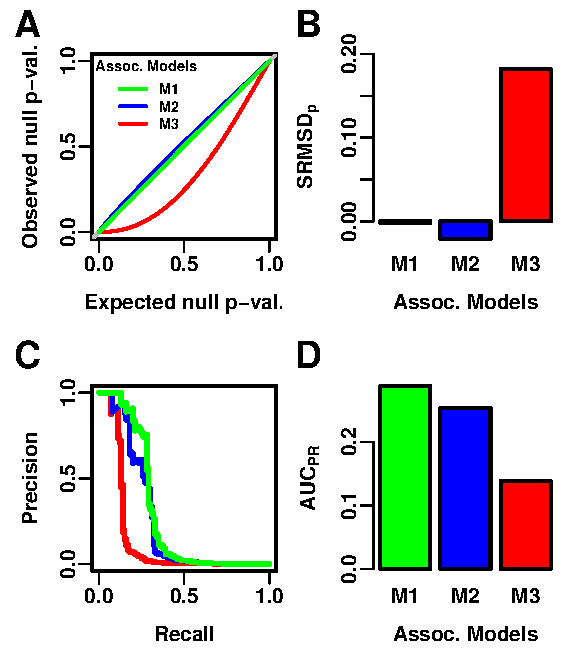
\includegraphics{sim-n1000-k10-f0.1-s0.5-g1/measures-illustration.pdf}
  \caption{
    {\bf Illustration of $\rmsd$ and $\auc$ evaluation measures.}
    Three archetypal models (M1, M2, M3) illustrate our two complementary measures.
    M1 is an ideal model that performs best overall, M2 overcorrects for population structure so it incurs a small performance penalty, and M3 does not correct for population structure so it performs most poorly.
    \textbf{A.}
    Probability-probability plot of the subset of p-values testing ``null'' (non-causal) loci.
    M1 has uniform null p-values as desired (overlaps $y=x$).
    M2/M3 have null p-values larger/smaller than expected.
    \textbf{B.}
    The $\rmsd$ (p-value Signed Root Mean Square Deviation) summarizes null p-value accuracy using a scaled Euclidean distance between the observed null p-values and their uniform expectation, with a negative sign if the median is larger than expected (closer to zero is better).
    \textbf{C.}
    Precision-Recall plot assesses classification prediction performance across significance thresholds, without assuming that p-values are accurate (only locus ranks matter; higher is better).
    \textbf{D.}
    The $\auc$ (Precision-Recall Area Under the Curve) summarizes predictive performance (higher is better).
  }
  \label{fig:measures_illustration}
\end{figure}

% PCA, LMM, PCs series
The overall goal is to characterize the performance of two association models: PCA and LMM.
Each of PCA and LMM was evaluated in each dataset while including a number $r$ of PCs as fixed covariates, in both cases varying $r$ between 0 and 90.
We determined which value of $r$ was optimal (in terms of $\rmsd$ and $\auc$ separately) for each of PCA and LMM separately, in each dataset, and lastly compared overall performance per dataset across the best PCA and LMM cases (with their optimal $r$ values).
Our overall statistical evaluation is presented in \cref{tab:human_sum_pcs} and will be summarized first, followed by detailed evaluations in each datasets in the rest of the results.

\begin{table}[hb!]
  \centering
  %\scriptsize
  \caption{
    \textbf{Overview of PCA and LMM evaluation results}
  }
  \label{tab:human_sum_pcs}
  \csvreader[
  tabular = lc|ccc|ccc,
  separator = tab,
  table head = 
  % header row 1
  \toprule & Metric: & \multicolumn{3}{c|}{$|\rmsd|$} & \multicolumn{3}{c}{$\auc$} \\
  % header row 2
  \midrule & & \multicolumn{2}{c}{Best (min\textsuperscript{b}) PCs} & & \multicolumn{2}{c}{Best (min\textsuperscript{b}) PCs} & \\
  % header row 3
  Dataset & {Trait model\textsuperscript{a}} & PCA & LMM & {Best\textsuperscript{c}} & PCA & LMM & {Best\textsuperscript{c}} \\\midrule,
  late after last line = \\\bottomrule
  ]{../data/stats.txt}{}{\csvlinetotablerow}
  \begin{flushleft}
    \textsuperscript{a}FES: Fixed Effect Sizes, RC: Random Coefficients.\\
    \textsuperscript{b}Smallest $r$ (number of PCs) whose distribution ($|\rmsd|$ or $\auc$) was not significantly different (Wilcoxon paired 1-tailed $p > 0.01$) from the $r$ with best mean value (if any). \\
    \textsuperscript{c}Tie if distributions ($|\rmsd|$ or $\auc$) of best PCA and LMM version (previous two columns) did not differ significantly (Wilcoxon paired 1-tailed $p > 0.01$).
    Result was always the same whether ``best'' or ``min'' (in parenthesis) cases were compared, except in one case (in parenthesis).\\
    *$r$ for which mean $|\rmsd| < 0.01$ ($|\rmsd|$ columns only).
  \end{flushleft}
\end{table}

We first describe the results for null p-value uniformity ($|\rmsd|$; \cref{tab:human_sum_pcs}).
Only here the sign of $\rmsd$ was ignored, so smaller is better and Wilcoxon paired 1-tailed tests were used to determine whether a suboptimal distribution was significantly different.
For PCA, the optimal number of PCs $r$ is typically very large across all datasets (up to $r=90$, which was the largest value tested), but we found that much smaller ``min'' $r$ values often performed as well (numbers in parentheses in \cref{tab:human_sum_pcs} are the smallest $r$ whose $|\rmsd|$ distributions were not significantly different from the distribution of the $r$ with the smallest mean $|\rmsd|$).
However, even the min $r$ values for PCA tended to be large on the family simulations and the real datasets, compared to the admixture and tree simulations.
In most cases both the best $r$ and the min $r$ had a mean $|\rmsd| < 0.01$ (marked with asterisks), indicating small enough effect sizes to consider those null p-value distributions effectively uniform.
Mean $|\rmsd| > 0.01$ cases for PCA also tended to be observed on the family simulations and real datasets.
In contrast, for LMM $r=0$ (no PCs) was always the optimal choice (always resulted in the minimum mean $|\rmsd|$), and in those cases we also always had mean $|\rmsd| < 0.01$.
Lastly, we compared the $|\rmsd|$ distributions between PCA and LMM, each with their best $r$, resulting in LMM besting often or in statistical ties, whereas PCA was best in the Human Origins simulations only.

Next we turn to the predictive power evaluations ($\auc$; \cref{tab:human_sum_pcs}).
For PCA, the best $r$ for $\auc$ was always smaller than the best $r$ for $|\rmsd|$, and also for the respective ``min'' $r$ comparisons (smallest $r$ which is not significantly different in $\auc$ distribution from the best $r$).
So for PCA there is often a tradeoff between the desire for accurate p-values versus maximizing power.
For LMM there is no such tradeoff, as $r=0$ (no PCs) resulted in $\auc$ distributions not significantly different from the best $r$ in all tests except one (in the 1000 Genomes simulation with the random coefficients trait model, the min $r$ was 1).
Lastly, LMM with its best $r$ always had significantly greater $\auc$ distributions than PCA with its best $r$.

\subsection{Evaluations in admixture simulations}

Now we look more closely at the results of every individual evaluation.
The measured $\rmsd$ and $\auc$ distributions, for each PCA and LMM and for each value of the number of PCs $r$, for the first three admixture simulations and the \textit{fixed effect size} trait simulation, are in \cref{fig:rmsd-auc-sim}.
We repeated the evaluation with traits simulated from the \textit{random coefficients} model as well, which gave qualitatively similar results (\cref{fig:rmsd-auc-sim-rc}).

The large admixture simulation has $n = 1,000$ individuals, and differs from previous admixture evaluations in featuring a larger number of ancestral populations ($K=10$) and more differentiation ($\Fst = 0.1$ for the admixed individuals).
Admixture is structured over a one-dimensional geography \citep{ochoa_estimating_2021}.
The $\rmsd$ of PCA is largest when $r=0$ (no PCs) and decreases rapidly to zero at $r=3$, where it stays for up to $r=90$ (\cref{fig:rmsd-auc-sim}A).
Thus, PCA gives effectively accurate p-values for all $r \ge 3$, which is surprisingly smaller than the theoretical optimum we expected for this simulation of $r = K - 1 = 9$.
In contrast, the $\rmsd$ distribution for LMM starts near zero for $r=0$, and as $r$ increases moves away from zero in the negative direction (null test statistics are deflated rather than inflated, so p-values become conservative).
The $\auc$ distribution of PCA is similarly worst at $r=0$, increases rapidly and peaks at $r = 3$, then decreases slowly for $r > 3$.
Similarly, the $\auc$ distribution for LMM starts near its maximum at $r=0$, and decreases overall for larger $r$.
Although the $\auc$ distributions for LMM and PCA overlap considerably for each $r$, LMM with $r=0$ has significantly greater $\auc$ values than PCA with $r=3$ (\cref{tab:human_sum_pcs}).
However, qualitatively PCA closely matches LMM in performance in this simulation.
It is also remarkable how robust both LMM and PCA are to greatly mispecifying $r$.

\begin{figure}[bp!]
  \centering
  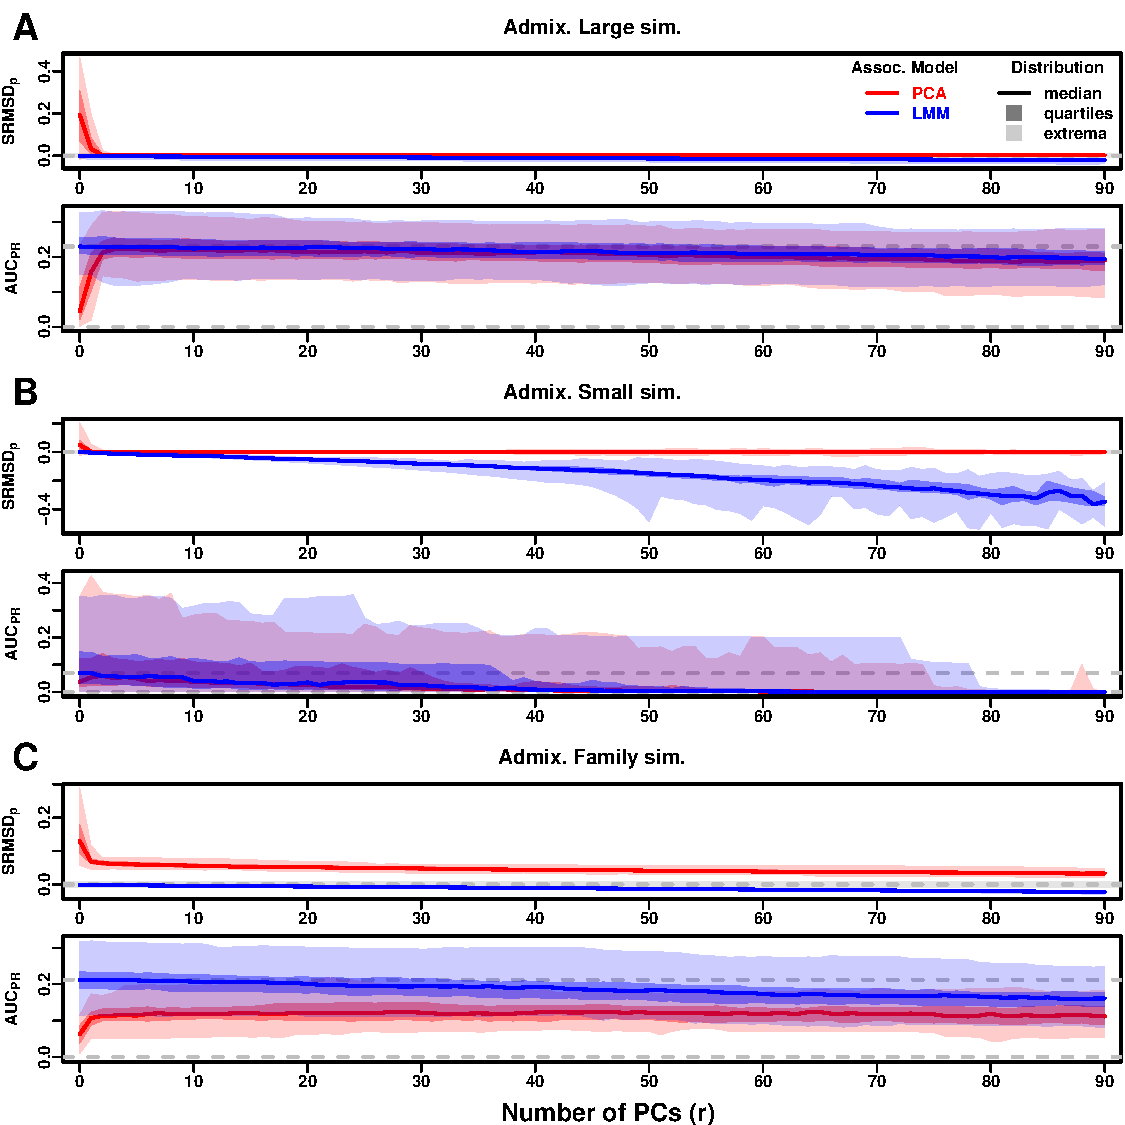
\includegraphics[width=\textwidth,height=\textheight,keepaspectratio]{fes/rmsd-auc-sim.pdf}
  \caption{
    {\small 
      {\bf Evaluations in admixture simulations.}
      Traits simulated from \textit{fixed effect sizes} model.
      PCA and LMM approaches are tested under varying number of PCs ($r \in \{0, ..., 90\}$ on x-axis), with the distributions (y-axis) of $\rmsd$ (top subpanel) and $\auc$ (bottom subpanel) for 50 replicates.
      Best performance is zero $\rmsd$ and large $\auc$.
      Zero values and maximum median $\auc$ values are marked with horizontal gray dashed lines, and the $|\rmsd| < 0.01$ band is marked with a light gray area.
      LMM always performs best when $r=0$, and PCA performs best when $r$ is between 1-4.
      \textbf{A.}
      The large simulation has $n = 1,000$ individuals.
      \textbf{B.}
      The small simulation has $n = 100$ individuals, helps illustrate overfitting for large $r$.
      \textbf{C.}
      The family simulation has $n = 1,000$ individuals from a family with admixed founders and large numbers of pairs of sibling, first/second cousins, etc, from a realistic random 20-generation pedigree.
      Here PCA performs poorly compared to LMM: $\rmsd > 0$ for all $r$, and a large gap in $\auc$.
    }
  }
  \label{fig:rmsd-auc-sim}
\end{figure}

The previous robustness to large $r$ led us to consider smaller sample sizes.
Our expectation is that a model with large numbers of parameters $r$ should overfit more as $r$ increases, and particularly as $r$ approaches the sample size $n$ (number of individuals).
Rather than increase $r$ beyond 90, which is not done in practice, we reduce to $n = 100$ individuals, which is small for typical association studies but may occur in studies of rare diseases, for pilot studies, or be due to low budgets or other constraints.
To compensate for the loss of power due to reducing $n$, we also reduce the number of causal loci from 100 before to $m_1 = 10$, (in all cases a fixed ratio of $n / m_1 = 10$) which increases the magnitude of each individual causal coefficient per locus.
As expected, here we found rapid decreases in performance for both PCA and LMM as $r$ increases, with optimal performance attained near $r=1$ for PCA and $r=0$ for LMM (\cref{fig:rmsd-auc-sim}B).
However, the shift to negative $\rmsd$ values for LMM as $r$ increases is much greater in this case.
The evaluation declares LMM with $r=0$ significantly better than PCA ($r=1$ to 4) in both metrics (\cref{tab:human_sum_pcs}), although qualitatively there is a negligible difference between the two models.

The last of the first three simulations adds a 20-generation random family to our admixture simulation.
Previous work has reported, in limited settings, that PCA performs poorly in the presence of family structure, so it is important to establish the detailed behavior of PCA and LMM in this setting as $r$ is varied for both.
Since the LMM is formulated in terms of kinship matrices, it is expected to perform better here.
Only the last generation is studied for association, which contains numerous siblings, first cousins, etc.
The initial population structure due to admixture is preserved across the generations by strongly biasing mating pairs for proximity over the one-dimensional geography, which results in an indirect ancestry-biased assortative mating (see Methods).
Our evaluation reveals a sizable gap in both metrics between LMM and PCA across all values of $r$ (\cref{fig:rmsd-auc-sim}C).
Thus, although LMM again performs best with $r=0$ and achieves mean $|\rmsd| < 0.01$, PCA does not achieve zero $\rmsd$ at any $r$ value (all p-values are strongly anti-conservative), and the best mean $\auc$ value across $r$ for PCA is worse than the worst mean $\auc$ value for LMM.
Thus, LMM is conclusively superior to PCA, and the only adequate model, when there is family structure.

\subsection{Evaluations in real human genotype datasets}

We were next interested in recapitulating our previous results using real human genotype data, which will give the most relevant results in practice, and which differs from our simulations in many ways, including marginal allele frequency distributions, potentially more complex population structures with greater differentiation, correlated and more numerous ancestral subpopulations, as well as the potential presence of cryptic family relatedness.
We chose three non-redundant datasets that span global human diversity and include both array and WGS genotyping technologies.
Loci in high linkage disequilibrium were removed to simplify our evaluation, and traits were simulated from these genotypes and each of the two trait models: fixed effect sizes (\cref{fig:rmsd-auc-real}) and random coefficients (\cref{fig:rmsd-auc-real-rc}).

Among the real datasets, Human Origins has the greatest number and diversity of subpopulations.
The $\rmsd$ and $\auc$ distributions in this dataset and the fixed effect sizes trait model (\cref{fig:rmsd-auc-real}A) most resemble those from the family simulation (\cref{fig:rmsd-auc-sim}C), which is surprising since close relatives are excluded from this data.
In particular, while LMM with $r=0$ again performed optimally (both metrics) and satisfies mean $|\rmsd| < 0.01$, PCA maintained mean $\rmsd > 0$ for all $r$ values and its $\auc$ values were all strictly smaller than even the worst $\auc$ values of LMM at any $r$.

\begin{figure}[bp!]
  \centering
  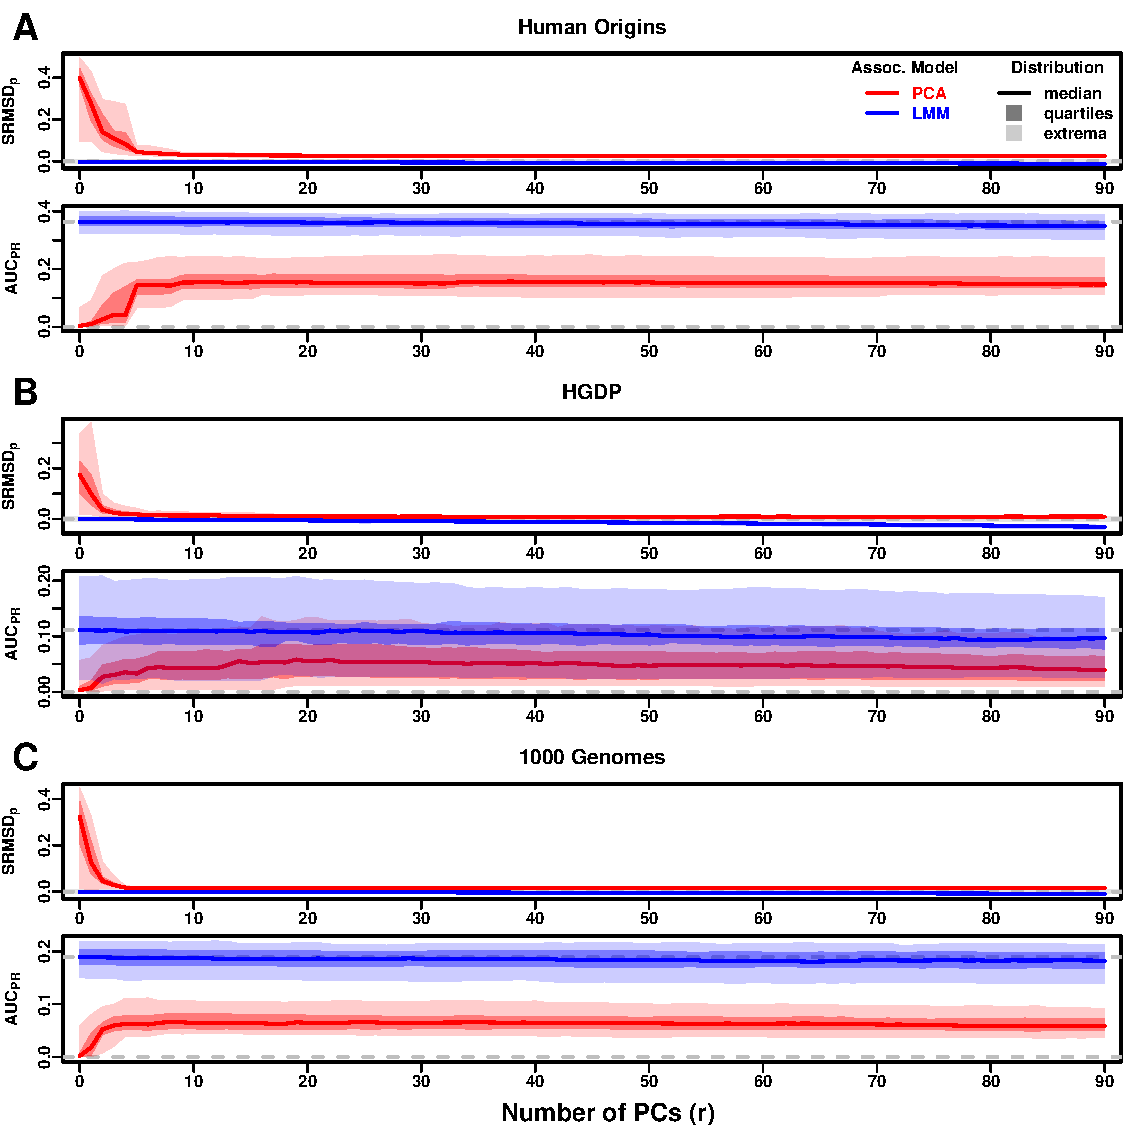
\includegraphics[width=\textwidth,height=\textheight,keepaspectratio]{fes/rmsd-auc-real.pdf}
  \caption{
    {\small 
      {\bf Evaluations in real human genotype datasets.}
      Traits simulated from \textit{fixed effect sizes} model.
      Same setup as \cref{fig:rmsd-auc-sim}, see that for details.
      These datasets strongly favor LMM with $r = 0$ PCs over PCA, resulting in curves that resemble the previous admixed family simulation, even though these datasets excluded known family members.
      \textbf{A.}
      The Human Origins dataset.
      \textbf{B.}
      The Human Genome Diversity Panel (HGDP) dataset.
      \textbf{C.}
      The 1000 Genomes Project dataset.
    }
  }
  \label{fig:rmsd-auc-real}
\end{figure}

The HGDP dataset has the fewest individuals among real datasets, which are a subset of Human Origins individuals that was recently genotyped with WGS, so it contains many more loci and has more rarer variants.
The $\rmsd$ and $\auc$ distributions (\cref{fig:rmsd-auc-real}B) are intermediate between the admixture and family simulations.
In particular, here both LMM ($r=0$) and PCA ($r \ge 31$) achieve mean $|\rmsd| < 0.01$, so null p-values will be accurate in both association models.
However, there is a sizable mean $\auc$ gap between LMM, which performed best across all values of $r$, and PCA.
Maximum $\auc$ values were lowest in HGDP compared to the two other human datasets.

1000 Genomes has the fewest subpopulations, but an intermediate number of individuals, compared to the other two real datasets, and like HGDP is also WGS.
Thus, although this dataset is expected to have the simplest population structure among the real datasets, we were surprised to find $\rmsd$ and $\auc$ distributions (\cref{fig:rmsd-auc-real}C) that again resemble those of our earlier family simulation, with mean $|\rmsd| < 0.01$ for LMM only and large $\auc$ gaps between LMM and PCA.

The previous results for the real datasets focused on traits drawn from the fixed effect sizes (FES) model.
In this case the results are qualitatively very different for traits drawn from the random coefficients (RC) model (\cref{fig:rmsd-auc-real-rc}).
The key difference is that $\auc$ gaps between LMM and PCA, which were very large in FES, are much smaller in RC.
Maximum $\auc$ were smaller in RC compared to FES in two of the three datasets.
$\rmsd$ distributions are practically the same in RC versus FES.
Nevertheless, our overall statistical evaluations declare LMM with $r=0$ superior to PCA in both RC and FES traits (\cref{tab:human_sum_pcs}).

\subsection{Evaluations in tree simulations fit to human data}

To better understand what features of the real datasets lead to the large differences in performance between LMM and PCA, we performed additional simulations.
In particular, human subpopulations are related roughly by a tree, which induces the strongest correlations by magnitude (\cref{fig:kinship}), so we wanted to determine if this tree structure alone could recapitulate our previous results.
Thus, we fit trees to each human dataset and verified that the kinship matrices of the simulations were a rough match to those of the real datasets, as desired.
The second feature included in these simulations (absent in the original admixture simulations) is a non-uniform ancestral allele frequency distribution, which recapitulated some of the skew for smaller minor allele frequencies of the real datasets (\cref{fig:kinship}C).

The $\rmsd$ and $\auc$ distributions for the tree simulations fit to the human data (\cref{fig:rmsd-auc-real-sim}) resembled our previous admixture simulation much more than either the family simulation (\cref{fig:rmsd-auc-sim}) or real data results (\cref{fig:rmsd-auc-real}).
In all three simulations, both LMM with $r=0$ and PCA (various $r$) achieve mean $|\rmsd| < 0.01$, and in two out of the three cases both association models (with their best $r$) were tied (not significantly different; \cref{tab:human_sum_pcs}).
The $\auc$ distributions of both LMM and PCA track closely as $r$ is varied, although there is a small gap in performance that results in LMM ($r=0$) besting PCA in all three simulations.
Lastly, the results are qualitatively similar for traits drawn from the random coefficients model (\cref{fig:rmsd-auc-real-sim-rc,tab:human_sum_pcs}).
Overall, the tree simulations do not recapitulate the large LMM advantage over PCA observed in the previous real human data results.

\begin{figure}[bp!]
  \centering
  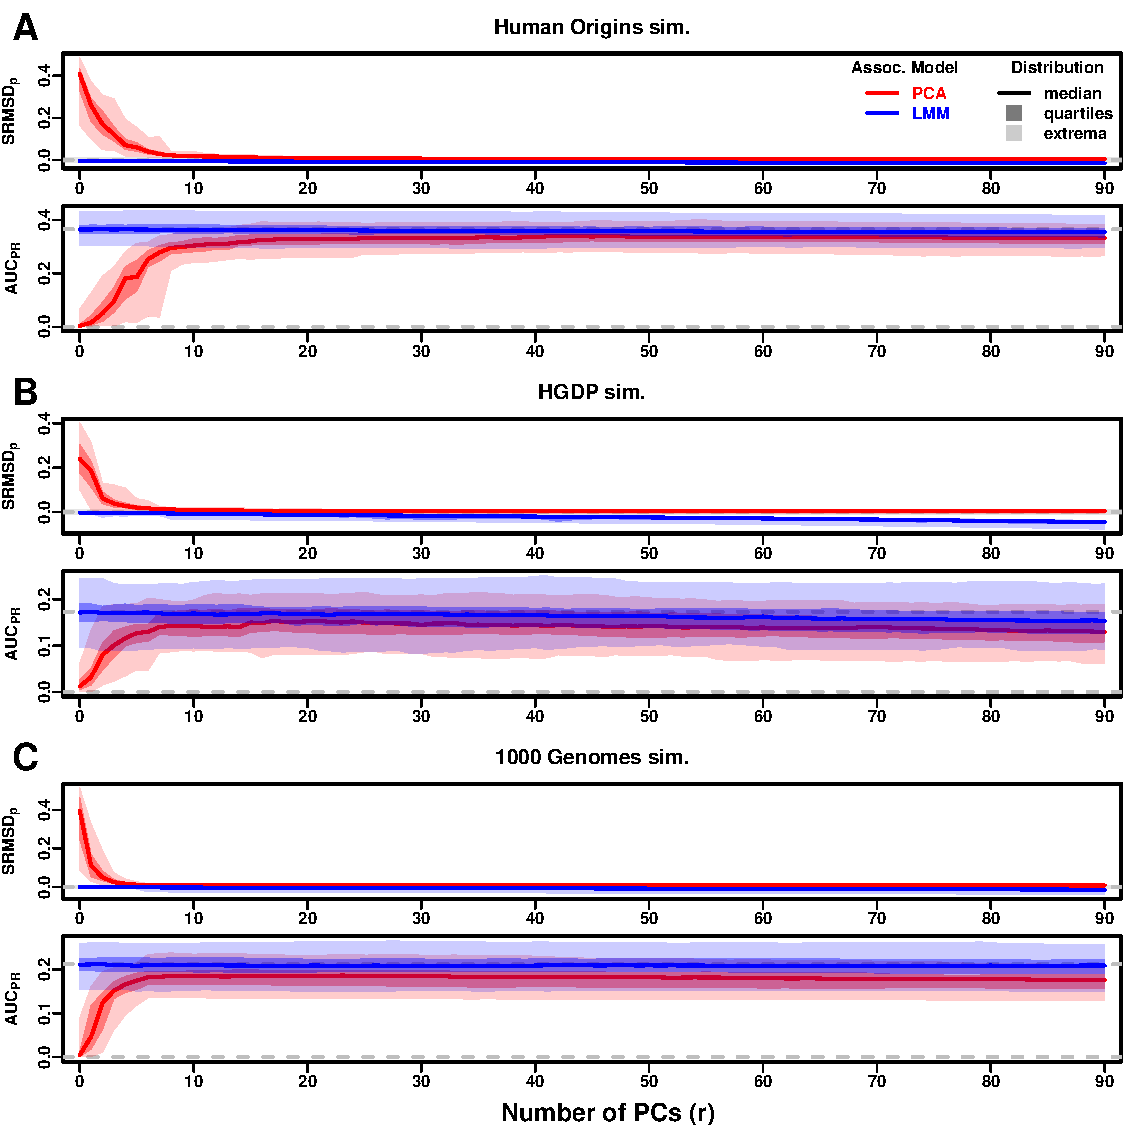
\includegraphics[width=\textwidth,height=\textheight,keepaspectratio]{fes/rmsd-auc-real-sim.pdf}
  \caption{
    {\small 
      {\bf Evaluations in tree simulations fit to human data.}
      Traits simulated from \textit{fixed effect sizes} model.
      Same setup as \cref{fig:rmsd-auc-sim}, see that for details.
      These tree simulations, which exclude within-subpopulation structure by design, do not explain the large gaps in LMM-PCA performance observed in the real datasets.
      \textbf{A.}
      The Human Origins simulation.
      \textbf{B.}
      The Human Genome Diversity Panel (HGDP) simulation.
      \textbf{C.}
      The 1000 Genomes Project simulation.
    }
  }
  \label{fig:rmsd-auc-real-sim}
\end{figure}

\subsection{Estimated eigenvalues do not explain PCA performance}

A first-principles hypothesis for why PCA performs well in some datasets and not in others is their differences in dimensionality, since PCA assumes a low-dimensional genetic structure whereas LMM can model high-dimensional genetic structures.
We applied the Tracy-Widom statistical test \citep{patterson_population_2006} with $p < 0.01$ to determine the number of significant principal components in each dataset, which estimates the rank of the kinship matrix (i.e., its dimensionality).
These kinship ranks (\cref{fig:eigen}A) slightly underestimated the true dimensionality of our simulations (\cref{tab:human_sum}).
However, rank estimates agree that the admixed family simulation has a greater rank than the admixture-only simulation, and that the real datasets have a much greater rank than the admixture simulations and (to a lesser extent) than the tree simulations that were fit to each real dataset (\cref{fig:eigen}A).
However, these estimated ranks do not differentiate datasets where PCA performs well from those where performance was poor.
For example, the ranks of the Human Origins and HGDP tree simulations, were PCA performed relatively well (\cref{fig:rmsd-auc-real-sim}), are much larger than the rank of the family simulation, where PCA performed very poorly (\cref{fig:rmsd-auc-sim}).
Moreover, the 1000 Genomes rank estimate is lower than 90, yet PCA performed poorly for all $r \ge 90$ numbers of PCs tested (\cref{fig:rmsd-auc-real}).
Performance might depend on the ratio of the matrix rank to its dimension (the number of individuals) or a more complicated formula, but the datasets tested do not differ greatly in dimensions (at most 3x, excluding the small simulation), while our analysis does not reveal an obvious line that separates these dataset by PCA performance.

\begin{figure}[bp!]
  \centering
  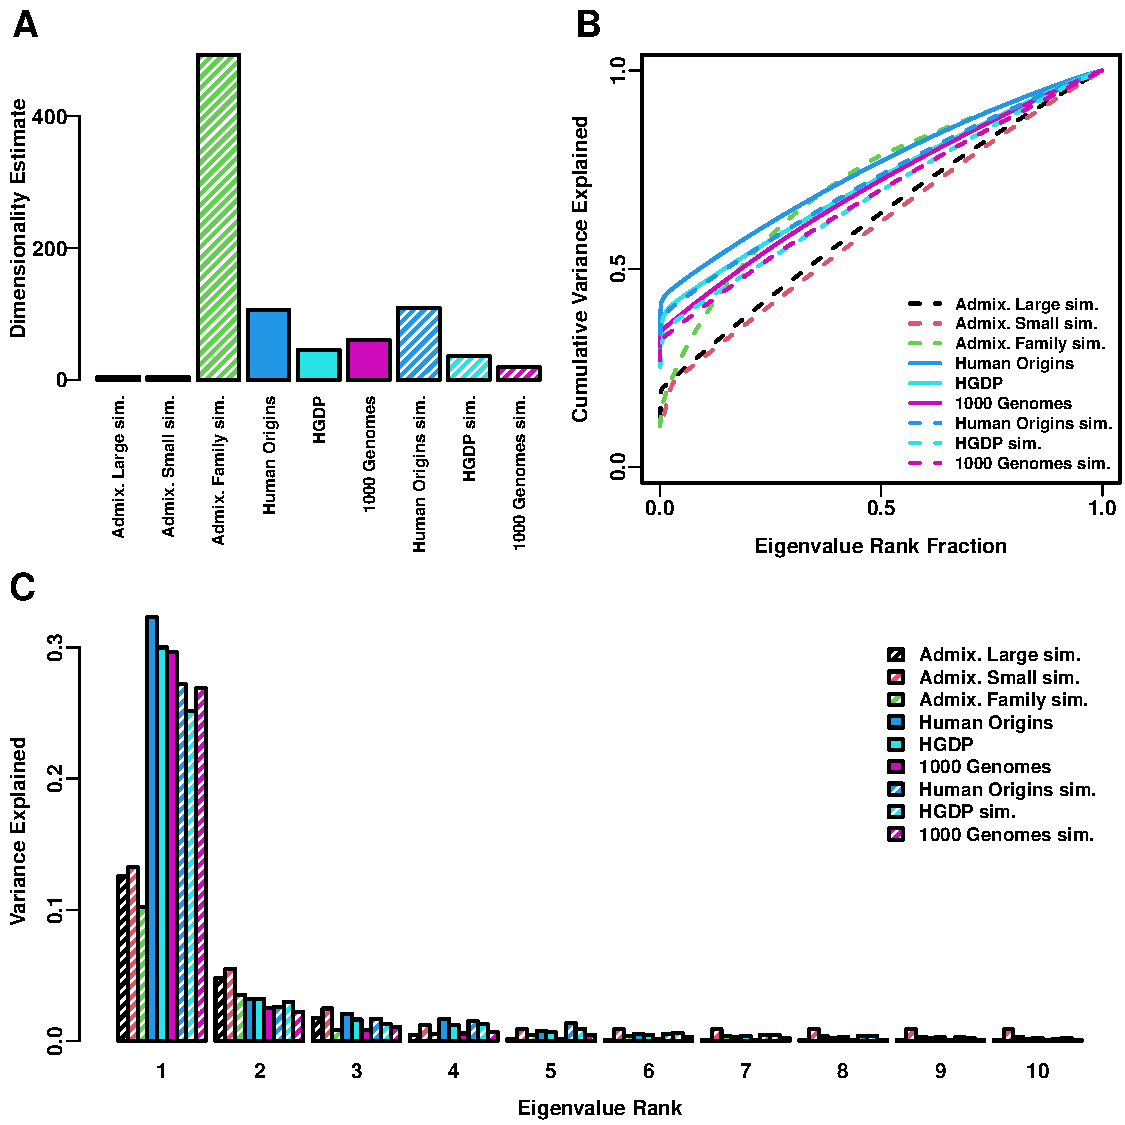
\includegraphics[width=\textwidth]{eigen.pdf}
  \caption{
    {\bf Estimated dimensionality of datasets.}
    \textbf{A.}
    Kinship matrix ranks estimated with the Tracy-Widom test with $p < 0.01$.
    \textbf{B.}
    Cumulative variance explained versus eigenvalue rank fraction ($i/n$ where $i$ is rank, $n$ is number of eigenvalues/individuals).
    \textbf{C.}
    Variance explained by first 10 eigenvalues.
  }
  \label{fig:eigen}
\end{figure}

We also compared eigenvalues across datasets, expressed as variance explained (each eigenvalue divided by the sum of eigenvalues) to facilitate comparisons across datasets.
The top eigenvalue explained a proportion of variance roughly proportional to \Fst (\cref{tab:human_sum}), but the rest of the top 10 eigenvalues show no large differences between datasets (\cref{fig:eigen}C), except the small admixture simulation had larger variances explained per eigenvalue (as expected since it has fewer of them).
We also visualized all eigenvalues (beyond the top 10), computing their cumulative variance explained distributions versus their eigenvalue rank fraction (normalized to account for dataset sample size differences).
Each dataset has a different starting point, but all increase almost linearly from there until they reach 1, except for the admixed family simulation, which has much greater variance explained by mid-rank eigenvalues (\cref{fig:eigen}B).
However, there are again no obvious clues separating datasets where PCA performed poorly (such as the real datasets) from those where it performed relatively well (such as the corresponding tree simulations).


\subsection{Comparison between $\rmsd$ and inflation factor}

Now that our main evaluation of the PCA and LMM models is concluded, we switch gears to a comparison of our new $\rmsd$ measure and the more traditional inflation factor common in the field.
The inflation factor $\lambda$ measures test statistic inflation, which is a way to measure total or residual population structure \citep{price_new_2010}.
We measured both measures in all of our evaluations, which enables us to discover a correspondence which we fit to all of our data.

Across our tests, we computed inflation factors by mapping median p-values back to their $\chi^2$ quantiles and comparing those values to their expectations under the null hypothesis (see Methods).
Remarkably, there appears to be a near one-to-one correspondence between these inflation factors $\lambda$ and our $\rmsd$ statistics (\cref{fig:rmsd_lambda}).
The curves for PCA and LMM models differ in sign: PCA tended to be inflated ($\lambda > 1$ and $\rmsd > 0$) whereas LMM tended to be deflated ($\lambda < 1$ and $\rmsd < 0$; not shown).
Other than that, it appears that the statistics for both PCA and LMM fall on the same contiguous curve.
One immediate advantage of $\rmsd$ over $\lambda$ is that the former does not take on as large values as the latter, which we had to plot on a log scale in \cref{fig:rmsd_lambda}.

\begin{figure}[bp!]
  \centering
  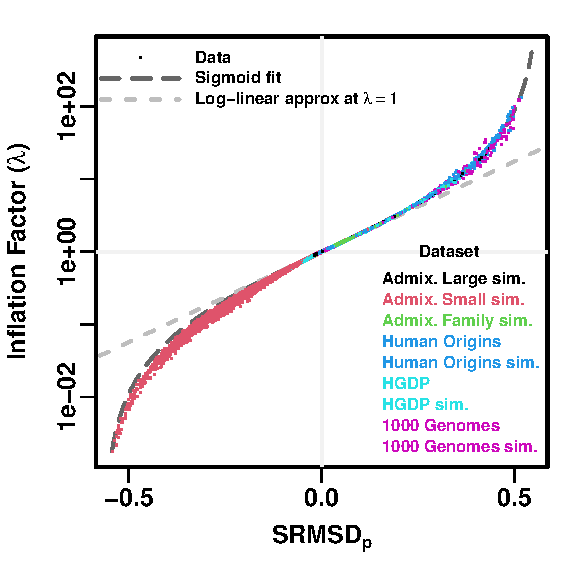
\includegraphics{sum-rmsd-vs-lambda.pdf}
  \caption{
    {\bf Comparison between $\rmsd$ and inflation factor.}
    These statistics were pooled from every number of PCs $r$ of both PCA and LMM models, both trait models, and every dataset (color coded by dataset).
    Note y-axis ($\lambda$) is on a log scale, while x-axis ($\rmsd$) is linear scale.
    The sigmoidal curve corresponds to \cref{eq:rmsd_lambda_sigmoidal}, and the log-linear approximation to \cref{eq:rmsd_lambda_log_linear}.
  }
  \label{fig:rmsd_lambda}
\end{figure}

We fit a sigmoidal curve to this data in order to further characterize the connection between $\lambda$ and $\rmsd$.
The family of functions we considered was
\begin{equation}
  \label{eq:rmsd_lambda_sigmoidal}
  \rmsd( \lambda ) = a \frac{ \lambda^b - 1 }{ \lambda^b + 1 },
\end{equation}
% inverse:
% lambda <- ( ( a + rmsd ) / ( a - rmsd ) )^(1/b)
which for all values of the parameters $a > 0$ and $b > 0$ satisfies $\rmsd( \lambda = 1 ) = 0$ and reflects $\log( \lambda )$ about zero ($\lambda = 1$) as desired from visual inspection, namely that
$$
\rmsd( \log( \lambda ) = -x ) = - \rmsd( \log( \lambda ) = x ).
$$
% \rmsd
% = a \frac{ e^{-bx} - 1 }{ e^{-bx} + 1 }
% = a \frac{ 1 - e^{bx} }{ 1 + e^{bx} }
We fit this model to the upper portion of the data only ($\lambda > 1$), since it was less noisy and of greater interest, and obtained the curve shown in \cref{fig:rmsd_lambda} with parameters $a = 0.566$ and $b = 0.616$.
Using this model, we also produced a log-linear approximation based on its Taylor series with respect to $x = \log( \lambda )$ about $x=0$, resulting in
\begin{equation}
  \label{eq:rmsd_lambda_log_linear}
  \rmsd( \lambda ) \approx \frac{a b}{2} \log( \lambda ),
\end{equation}
% inverse:
% lambda <- exp( 2 * rmsd / ( a * b ) )
which is also shown in \cref{fig:rmsd_lambda}.
The value $\lambda = 1.05$, a threshold typically used to determine that there is no inflation \citep{price_new_2010}, corresponds to $\rmsd = 0.0085$ according to both \cref{eq:rmsd_lambda_sigmoidal,eq:rmsd_lambda_log_linear}.
Conversely, $\rmsd = 0.01$, serving as a simpler rule of thumb, corresponds to $\lambda = 1.06$ according to both formulas too.


\section{Discussion}

Our evaluations conclusively determined that LMM without PCs performs better than PCA (for any number of PCs) across all scenarios, including all real and simulated genotypes and two trait simulation models.
Although the addition of a few PCs does not greatly hurt the performance of LMM (except when sample sizes are very small), such additions never resulted in significantly improved perfomance either (barring one marginally significant case with a small effect size; \cref{tab:human_sum_pcs}), which aggrees with previous observations \citep{liu_controlling_2011} but contradicts others \citep{zhao_arabidopsis_2007, price_new_2010}.
Our findings make sense since the PCs are the eigenvectors of the kinship matrix used to model the random effects, so including both is redundant.

Previous work also suggested that PCA can outperform LMM when [TODO: harmonize with intro] there are loci under selection or otherwise highly differentiated \citep{price_new_2010, wu_comparison_2011, yang_advantages_2014}.
Our evaluations on real human data, which presumably contain such loci in realistic proportions, if they are realistic scenarios at all, do not replicate those observations.
However, the probable presence of cryptic relatedness on all of these datasets (see below), which favors LMM, may obscure the expected effect.
Therefore, while we are not able to completely dismiss this potential PCA advantage, it probably plays a minor role in human studies.

Relative to LMM, the behavior of PCA fell into two extremes.
When PCA performed well, there was a (typically small) number of PCs that resulted in both near zero mean $\rmsd$ and mean $\auc$ near that of LMM without PCs.
Conversely, when PCA performed poorly, no choice for the number of PCs led to either acceptably low $\rmsd$ or acceptably large $\auc$.
PCA performed well in the admixture simulations (without families, both trait models), real human genotypes with random coefficients traits, and, to a lesser extent, the tree simulations (both trait models).
Conversely, PCA performed poorly in the admixed family simulation (both trait models) and the real human genotypes with fixed effect sizes traits.

PCA makes an inherent assumption that genetic structure is low-dimensional, whereas LMM can handle high-dimensional structures too.
Thus, PCA performs well in the admixture simulation, which is explicitly low-dimensional (see Methods), as well as in tree simulations with few nodes or few long branches, such as the trees we fit to the real human data, where a low-dimensional approximation is sufficient.
Conversely, PCA performs poorly under family structure because its kinship matrix is high-dimensional.
One theoretical inconvenience is that true kinship matrices are always full rank: for example, an unstructured population where all individuals are equally unrelated and outbred has a kinship matrix of $\mathbf{I}/2$, whose eigenvalues are all equal to $1/2$.
Nevertheless, population structure induces a more unbalanced eigenvalue distribution with a few very large eigenvalues (\cref{fig:eigen}), so we may define dimensionality in practice as the number of eigenvalues that exceed some small threshold.
However, evaluating the dimensionality of real datasets is challenging because estimated kinship/covariance matrices result in noisy eigenvalues with skewed distributions.
We used the Tracy-Widom test to estimate dimensionality \citep{patterson_population_2006}, which gives estimates coherent with the simulation models, although it slightly underestimated their dimensionality (as expected since some non-zero eigenvalues are too small to be significant at the given sample size, and are potentially also less important in practice as evident in our evaluations, as PCA often also performed best with many fewer PCs than the true simulation rank).
This analysis confirms that there is considerable structure in real human datasets, which have ranks that exceed the typical 10 PC used in practice and partly explains why LMM performs much better in those cases.
However, estimated eigenvalues and kinship matrix ranks by themselves do not fully explain when PCA will perform unacceptably poorly.
An additional complication that our evaluations reveal is that the model relating the trait to the genotypes also determines the relative performance of PCA, so genotype-based eigenvalues alone cannot tell the full story.

The real human genotype results, which are the most relevant in practice, suggests that PCA is at best underpowered relative to LMMs, and at worst produces inflated statistics regardless of the numbers of PCs included.
Among our simulations, such poor performance with the same features was observed only in the admixed family simulation, so our hypothesis is that cryptic relatedness explains our observations.
The very large differences in rank between each real dataset and its tree simulation, particularly for 1000 Genomes and HGDP, support our hypothesis that there is considerable high-dimensional relatedness not captured by the tree model.
Admixture is not modeled in our tree simulations, but our other admixture simulations concluded that this feature by itself is not problematic for PCA, so its exclusion should not affect PCA performance.
Therefore, by elimination, our analysis again points to cryptic relatedness as the culprit for poor PCA performance in real datasets.
Although each of those real human studies excluded individuals known to be related, reanalysis of 1000 Genomes has confirmed the presence of hundreds of close relative pairs (a few as close as siblings or parent-children; \cite{gazal_high_2015, al-khudhair_inference_2015, fedorova_atlas_2016, schlauch_identification_2017}).
However, it is unclear which scenarios lead to worse PCA performance, for example, between a few highly related individuals (which are easy to identify and remove) versus a large number of more distantly related pairs.
Nevertheless, cryptic relatedness is expected to be prevalent in any large human dataset \citep{henn_cryptic_2012, shchur_number_2018}.
In view of this evidence, it appears that the challenges of cryptic relatedness are exacerbated when rare variants have large coefficients, as they do in our fixed-effect-sizes trait model.
Thus, the high-dimensionality induced by cryptic relatedness appears to be the key challenge for PCA-based association in modern datasets that is readily overcome by LMM.

Minor conclusions follow.
Our extensive evaluation also determined that PCA is robust to using a large number of PCs, often far beyond the optimal choice, which agrees with previous anecdotal observations \citep{price_principal_2006, kang_variance_2010}.
This is in contrast to using too few PCs, for which there is a large performance penalty.
The only exception was the small simulation, where choosing just the right number of PCs was critical for performance.
Thus, when simulations such as ours are not feasible, it is best to err on the side of including too many PCs rather than risk including too few.
In this sense, LMM is also more straightforward as users need not select any parameters such as the number of PCs, which to do right requires additional work or knowledge.
Conversely, we found that if an LMM has a large number of covariates relative to its sample size (in our case PCs, though we expect this to generalize) then p-values become too conservative/deflated ($\rmsd$ was often negative across datasets when $r=90$), which is a weakness of LMM's use of the likelihood ratio test and its asymptotic $\chi^2$ distribution, which PCA overcomes with the more accurate t-test.
Post-hoc evaluations, or simulations such as ours, remain important in all cases to ensure that statistics are as expected, and may help decide whether to use PCA or LMM in a given setting.

Overall, our results force us to always recommend the use of LMM over PCA.
Although PCA offer flexibility and speed compared to LMM, additional work is required to ensure that PCA is adequate, including identifying close relatives for exclusion (lowering sample size and resulting in wasted resources) followed by simulations or other evaluations of the output statistics, and even then, without also running LMM there is no guarantee that PCA performance will be close enough to the improved power of LMM we observed in all of our evaluations.
Our findings also suggest that other applications that employ PCA to control for population structure, such as polygenic risk scores \citep{qian_fast_2020}, may enjoy gains in power by instead employing an LMM or some other high-dimensional population structure model capable of jointly modeling population structure and cryptic relatedness.
%This was one of the observations of a recent reevaluation of polygenic adaptation for height \citep{berg_reduced_2019}.

% Since PCA matches the performance of LMM when there is no family structure, this argues against the simple characterization that either fixed or random effects are in principle superior models for association studies \citep{price_new_2010, sul_mixed_2013, price_response_2013, sul_population_2018}.

%%% TODOTODOTODO

\section{Models and Methods}

\subsection{Models for genetic association studies}

In this subsection we describe the complex trait model and kinship model that motivates both the PCA and LMM models for genetic association studies, followed by further details regarding the PCA and LMM approaches.
The derivations of the PCA and LMM models from the general quantitative trait model are similar to previous presentations \citep{astle_population_2009, hoffman_correcting_2013}, but we emphasize the kinship model for random genotypes as being crucial for these connections, and make a clear distinction between the true kinship matrix and its most common estimator, which is biased \citep{ochoa_estimating_2021, ochoa_human}.

\subsubsection{The complex trait model and PCA approximation}

Let $\xij \in \{ 0, 1, 2 \}$ be the genotype at locus $i$ for individual $j$, which counts the number of reference alleles.
Suppose there are $n$ individuals and $m$ loci,
$\mathbf{X} = ( \xij )$ is their $m \times n$ genotype matrix, and
$\mathbf{y}$ is the length-$n$ (column) vector which represents trait value for each individual.
The approaches we consider are based on the following additive linear model for a quantitative (continuous) trait:
\begin{equation}
  \label{eq:trait}
  \mathbf{y}
  =
  \mathbf{1} \alpha + \mathbf{X}^\intercal \boldsymbol{\beta} + \boldsymbol{\epsilon}
  ,
\end{equation}
where
$\mathbf{1}$ is a length-$n$ vector of ones,
$\alpha$ is the scalar intercept coefficient,
$\boldsymbol{\beta}$ is the length-$m$ vector of locus coefficients,
$\boldsymbol{\epsilon}$ is a length-$n$ vector of residuals,
and the $\intercal$ superscript denotes matrix transposition.
The residuals are assumed to follow a normal distribution: $\epsilon_j \sim \text{Normal}(0, \sigma^2)$ independently for each individual $j$, for some residual variance parameter $\sigma^2$.

Typically the number of loci $m$ is in the order of millions while the number of individuals $n$ is in the thousands, or in other words, $m \gg n$.
Hence, the full model above cannot be fit in this typical case, as there are more parameters ($m+1$, the length of $\boldsymbol{\beta}$ and $\alpha$) than datapoints ($n$, the length of $\mathbf{y}$) to fit.
The PCA model with $r$ PCs approximates the full model fit at a single locus $i$:
\begin{equation}
  \label{eq:pca_gwas}
  \mathbf{y}
  =
  \mathbf{1} \alpha + \mathbf{x}_i \beta_i + \mathbf{U}_r \boldsymbol{\gamma}_r + \boldsymbol{\epsilon}
  ,
\end{equation}
where $\mathbf{x}_i$ is the length-$n$ vector of genotypes at locus $i$ only,
$\beta_i$ is the coefficient for that locus,
$\mathbf{U}_r$ is an $n \times r$ matrix of PCs, and
$\boldsymbol{\gamma}_r$ is the length-$r$ vector of coefficients for the PCs.
This approximation is explained by first noticing that the genotype matrix has the following singular value decomposition:
$\mathbf{X}^\intercal = \mathbf{U} \mathbf{D} \mathbf{V}^\intercal$,
where assuming $n < m$ we have that
$\mathbf{U}$ is an $n \times n$ matrix of the left singular vectors of $\mathbf{X}$,
$\mathbf{V}$ is an $m \times n$ matrix of its right singular vectors, and
$\mathbf{D}$ is an $n \times n$ diagonal matrix of its singular values.
Thus, in the full model we have
$\mathbf{X}^\intercal \boldsymbol{\beta} = \mathbf{U} \boldsymbol{\gamma}$,
where
$\boldsymbol{\gamma} = \mathbf{D} \mathbf{V}^\intercal \boldsymbol{\beta}$ is a length-$n$ vector.
The approximation consists solely of replacing $\mathbf{U} \boldsymbol{\gamma}$ (the full set of $n$ left singular vectors and their coefficients) with $\mathbf{U}_r \boldsymbol{\gamma}_r$ (the top $r$ singular vectors only, which constitutes the best approximation of rank $r$).
Thus, the extra terms in the PCA model approximate the polygenic effect of the whole genome, and assumes that the locus $i$ being tested does not contribute greatly to this signal.

\textbf{Statistical significance.}
The null hypothesis is $\beta_j = 0$ (no association).
The null and alternative models are each fit (fitting the coefficients of the multiple regression, where $\beta_j$ is excluded under the null while it is fit under the alternative).
The resulting regression residuals are compared to each other using the t-test, yielding a two-sided p-value.
Note that many common PCA implementations trade this t-test for a less accurate $\chi^2$ test, which requires the overall degrees of freedom of the model to be much smaller than the number of individuals.

% Genetic association studies are a multiple hypothesis testing problem, since there are a large number of loci ($m$) tested for association.
% In human genetic studies it has long been customary to set a p-value threshold of $5 \times 10^{-8}$ [TODO: citation], which may be thought of as controlling the total number of false discoveries, or equivalently, the family-wise error rate [TODO citations].
% The recommended solution to this problem in other fields is to control the FDR rather than setting a fixed p-value threshold.
% We recommend estimating q-values and setting a threshold of $q < 0.05$ so that the FDR is controlled at the 5\% level \citep{storey_positive_2003, storey_statistical_2003}.
% However, in this present work we do not calculate q-values; instead we focus on testing for the correctness of null p-value distributions (a prerequisite for acccurate q-value estimation) and on predictive power (for which ranking of loci by p-values suffice; q-values do not alter these rankings).

\subsubsection{Kinship model for genotypes}

In order to better motivate the most common estimation procedure of PCs for genotype data, and to connect PCA to LMMs, we shall review the kinship model for genotypes.
The model states that genotypes are random variables with a mean and covariance structure given by
$$
\E[ \xij | T ]
=
2 \pit,
\quad\quad
\Cov( \xij, \xij[k] | T )
=
4 \pit ( 1 - \pit ) \kt,
$$
where $T$ denotes the ancestral population quantities are conditioned upon, \pit is the ancestral allele frequency at locus $i$, and \kt is the kinship coefficient between individuals $j$ and $k$ \citep{malecot_mathematiques_1948, wright_genetical_1951, jacquard_structures_1970}.
Thus, if we standardize the genotype matrix using the true ancestral allele frequencies \pit, as
$$
\mathbf{X}_S
=
\left(
  \frac{
    \xij - 2 \pit
  }{
    \sqrt{4 \pit \left( 1 - \pit \right)}
  }
\right)
,
$$
then this results in a straightforward kinship matrix estimator:
$$
\E
\left[
\frac{1}{m}
\mathbf{X}_S^\intercal
\mathbf{X}_S
\right]
=
\mathbf{\Phi}^T
,
$$
where $\mathbf{\Phi}^T = ( \kt )$ is the $n \times n$ kinship matrix (do not confuse the ancestral population superscript $T$ with the matrix transposition symbol $\intercal$).
Replacing the raw genotype matrix $\mathbf{X}$ with the standardized matrix $\mathbf{X}_S$ in the trait model of \cref{eq:trait} results in an equivalent model, as this covariate differs only by a linear transformation.
Thus, under the standardized genotype model, the PCs of interest are equal in expectation to the top eigenvectors of the kinship matrix.

\subsubsection{Estimation of principal components from genotype data}

In practice, the matrix of principal components $\mathbf{U}_r$ in \cref{eq:pca_gwas} is calculated from an estimate of the earlier standardized genotype matrix $\mathbf{X}_S$, namely
\begin{equation*}
  \mathbf{\hat{X}}_S
  =
  \left(
    \frac{
      \xij - 2 \pith
    }{
      \sqrt{4 \pith \left( 1 - \pith \right)}
    }
  \right)
  ,
\end{equation*}
where the true ancestral allele frequency \pit is replaced by the estimate
$
\pith = \frac{1}{2n} \sum_{j = 1}^n \xij,
$
and results in the kinship estimate
\begin{equation}
  \label{eq:kinship_std}
  \mathbf{\hat{\Phi}}^T
  =
  \frac{1}{m}
  \mathbf{\hat{X}}_S^\intercal
  \mathbf{\hat{X}}_S
  .
\end{equation}
This kinship estimate and minor variants are also employed in LMMs \citep{yang_gcta:_2011}.
This estimator of the kinship matrix is biased, and this bias is different for every individual pair \citep{ochoa_estimating_2021, ochoa_human}.
However, in regression-based genetic association models such as PCA and LMM, the existing approach performs as well as when the above estimate is replaced by the true kinship matrix (data not shown).
The explanation, briefly, is that the biased expectation of the above estimator differs from the true kinship matrix by a rank-1 update, which is exactly compensated for by the intercept term $\mathbf{1} \alpha$ in \cref{eq:pca_gwas}.
[TODO: cite BIAS GWAS]

\subsubsection{Connection between PCs and ancestry proportions}

Here we show that genetic association using ancestry proportions as covariates is equivalent to using PCs.
We shall assume the following individual-specific admixture model commonly assumed when inferring ancestry proportions \citep{pritchard_inference_2000, falush_inference_2003, alexander_fast_2009, gopalan_scaling_2016, cabreros_likelihood-free_2019}.
There are $K$ subpopulations and every individual $j$ draws a proportion $q_{ju}$ of its alleles from subpopulation $S_u$.
These ancestry proportions must be non-negative and sum to one for every individual $j$ ($\sum_{u=1}^K q_{ju} = 1$ for every $j$).
Each subpopulation $S_u$ has an allele frequency $p_i^{S_u}$ at locus $i$, and thus the individual-specific allele frequency $\pi_{ij}$ of individual $j$ at locus $i$ is given by the weighted average of the subpopulation allele frequencies, where the ancestry proportions are the weights:
\begin{equation}
  \label{eq:admix}
  \pi_{ij} = \sum_{u=1}^K q_{ju} p_i^{S_u}.
\end{equation}
Genotypes are constructed by drawing each allele independently from this frequency, or $\xij | \pi_{ij} \sim \text{Binomial}(2, \pi_{ij})$.
% The $K$ subpopulations are assumed to be related by a general $K \times K$ coancestry matrix $\mathbf{\Psi}$ (each element $\psi_{uv}$ equals the kinship between random individual pairs, once from subpopulation $S_u$ and the other from $S_v$; the diagonal value $\psi_{uu}$ is both the kinship between any two different individuals in $S_u$ and the inbreeding coefficient of every individual in $S_u$).
Thus, the rowspace of the genotype matrix is, in expectation, the same as the rowspace of the individual-specific allele frequency matrix, which by \cref{eq:admix} above is the same as the rowspace of the $n \times K$ admixture proportions matrix $\mathbf{Q} = (q_{ju})$.
Therefore, the top $K$ principal components suffice to fully model the rowspace of the genotypes, which only have dimension $K$.
As an intercept term is always included in genetic association studies ($\mathbf{1} \alpha$ in \cref{eq:pca_gwas}), and the sum of rows of $\mathbf{Q}$ sums to one, then the rowspace of the combined model has dimension $K$ as well, so only $K-1$ PCs (plus intercept) are needed to span the rowspace of this admixture model.

\subsubsection{Linear mixed-effects model}

The LMM is another approximation to the complex trait model in \cref{eq:trait}.
Most LMM implementations support fixed covariates (how we combine LMM with PCs), but for simplicity they will be excluded in this presentation of the classical LMM, which is
\begin{equation}
  \label{eq:lmm_gwas}
  \mathbf{y}
  =
  \mathbf{1} \alpha + \mathbf{x}_i \beta_i + \mathbf{s} + \boldsymbol{\epsilon}
  ,
\end{equation}
which is like the PCA model in \cref{eq:pca_gwas} except that the PC terms $\mathbf{U}_r \boldsymbol{\gamma}_r$ are replaced by the random effect $\mathbf{s}$, which is a length-$n$ vector drawn from \citep{sul_population_2018}
$$
\mathbf{s} \sim \text{Normal} \left( \mathbf{0}, \sigma^2_s \mathbf{\Phi}^T \right),
$$
where $\mathbf{\Phi}^T$ is the kinship matrix and $\sigma^2_s$ is a trait-specific variance scaling factor.
This model is derived from treating the standardized genotype matrix $\mathbf{X}_S$ as random rather than fixed, so that the standardized genetic effect
$\mathbf{X}_S^\intercal \boldsymbol{\beta}_S$
in \cref{eq:trait} has mean zero and a covariance matrix of
$$
\Cov \left( \mathbf{X}_S^\intercal \boldsymbol{\beta}_S \right)
=
|| \boldsymbol{\beta}_S ||^2 \mathbf{\Phi}^T
.
$$
The above random effect $\mathbf{s}$ satisfies those equations, where the variance scale equals $\sigma^2_s = || \boldsymbol{\beta}_S ||^2$.
Thus, the PCA approach is the fixed model equivalent of the LMM under the additional approximation that only the top $r$ eigenvectors are used in PCA whereas the LMM uses all eigenvectors.
A more explicit comparison follows in the next subsection.

In practice, the key advantage of LMM over PCA is that it has fewer parameters to fit: ignoring the shared terms in \cref{eq:pca_gwas} and \cref{eq:lmm_gwas}, PCA has $r$ parameters to fit (each PC coefficient in the $\boldsymbol{\gamma}$ vector), whereas LMMs only fit one additional parameter, namely $\sigma^2_s$.
Therefore, PCA is expected to overfit more substantially than LMM---and thus lose power---when $r$ is very large, and especially when the sample size (the number of individuals $n$) is very small.
Statistical significance in LMMs most often employs a likelihood ratio test, whose test statistic has a asymptotic $\chi^2$ distribution under the null hypothesis.

\subsubsection{Connection between LMM and PCA models}

The LMM of \cref{eq:lmm_gwas} can be written to resemble more greatly the PCA model of \cref{eq:pca_gwas} \citep{astle_population_2009, hoffman_correcting_2013}, as
\begin{equation}
  \label{eq:lmm_gwas_evd}
  \mathbf{y}
  =
  \mathbf{1} \alpha + \mathbf{x}_i \beta_i + \mathbf{U} \boldsymbol{\gamma}_\text{LMM} + \boldsymbol{\epsilon}
  , \quad\quad
  \boldsymbol{\gamma}_\text{LMM} = \sigma_s \boldsymbol{\Lambda}^{1/2} \mathbf{r}
  ,
\end{equation}
where $\mathbf{U}$ is the complete matrix of PCs (all $n$ of them), $\boldsymbol{\Lambda}$ is the diagonal matrix of eigenvalues of the kinship matrix such that its eigendecomposition is $\mathbf{\Phi}^T = \mathbf{U} \boldsymbol{\Lambda} \mathbf{U}^\intercal$, and $\mathbf{r} \sim \text{Normal}(\mathbf{0},\mathbf{I})$ is a standard normal random effect.
The connection follows since $\mathbf{s} = \sigma_s \mathbf{U} \boldsymbol{\Lambda}^{1/2} \mathbf{r}$ satisfies
$$
\mathbf{s} \sim \text{Normal} \left( \mathbf{0}, \left( \sigma_s \mathbf{U} \boldsymbol{\Lambda}^{1/2} \right) \left( \sigma_s \mathbf{U} \boldsymbol{\Lambda}^{1/2} \right)^\intercal \right)
= \text{Normal}( \mathbf{0}, \sigma_s^2 \mathbf{\Phi}^T ),
$$
which itself follows from the affine transformation property of multivariate normal distributions.
Note that $\mathbf{U}$ also equals in the limit the right singular vectors of the standardized genotype matrix $\mathbf{X}_S = \mathbf{V}_S \mathbf{D}_S \mathbf{U}_S^\intercal$, which is how we originally motivated the PCA model, since
$$
\frac{1}{m} \mathbf{X}_S^\intercal \mathbf{X}_S
%= \frac{1}{m} \mathbf{U}_S \mathbf{D}_S \mathbf{V}_S^\intercal \mathbf{V}_S \mathbf{D}_S \mathbf{U}_S^\intercal
= \mathbf{U}_S \mathbf{\Lambda}_S \mathbf{U}_S^\intercal
\toas
\mathbf{U} \mathbf{\Lambda} \mathbf{U}^\intercal
=
\mathbf{\Phi}^T
$$
since $\mathbf{V}_S$ is orthonormal, and where $\mathbf{\Lambda}_S = \frac{1}{m} \mathbf{D}_S^2$.

Therefore, when the kinship matrix is low-dimensional (when only a few eigenvalues are very large), the LMM fits the same low-dimensional space as PCA would with an appropriate number of PCs, except that the coefficients $\boldsymbol{\gamma}_\text{LMM}$ are constrained by the likelihood model, whereas the analogous PCA coefficients $\boldsymbol{\gamma}_r$ are unconstrained variables.
On the other hand, when the kinship matrix is high-dimensional then the LMM can fit this space better than a corresponding PCA model with a small number of PCs, while PCA with a larger number of PCs will instead overfit the data.

\subsection{Simulations}

Here the general notation $\f{A}{B}$ denotes the inbreeding coefficient of a subpopulation $A$ from another subpopulation $B$ that is ancestral to $A$.
Often we use $\ft[A]$ where $T$ is an overall ancestral population (ancestral to every subpopulation and/or individual under consideration, such as the most recent common ancestor population).
[TODO: introduce more notation here, or do it all earlier?]

\subsubsection{Genotype simulation from the admixture model}

We consider three admixture simulation scenarios, refered to as Large, Small, and Family.
All cases are based on the admixture model described previously \citep{ochoa_fst1, ochoa_estimating_2021}.

The Large and Family simulations have $n = 1,000$ individuals, while Small has $n = 100$.
The number of loci in all cases is $m = 100,000$.
Individuals are admixed from $K = 10$ intermediate subpopulations.
Each subpopulation $S_u$ ($u \in \{ 1, ..., K \}$) has an inbreeding coefficient $\ft[S_u] = u \tau$, individual-specific admixture proportions $q_{ju}$ for individual $j$ and intermediate subpopulation $S_u$ arise from a random walk model for the intermediate subpopulations on a 1-dimensional geography with spread $\sigma$, where the free parameters $\tau$ and $\sigma$ are fit to result in $\Fst = 0.1$ for the admixed individuals and a bias coefficient of $s = 0.5$, as before \citep{ochoa_estimating_2021}.

Random allele frequencies and genotypes are drawn from the following hierarchical model:
\begin{align*}
  \pit
  &\sim
    \text{Uniform}( 0.01, 0.5 )
    , \\
  p_i^{S_u} | \pit
  &\sim
    \text{Beta} \left(
    \pit \left( \frac{1}{ \ft[S_u] } - 1 \right),
    \left( 1 - \pit \right) \left( \frac{1}{ \ft[S_u] } - 1 \right)
    \right)
    , \\
  \pi_{ij}
  &=
    \sum_{u = 1}^K q_{ju} p_i^{S_u}
    , \\
  \xij | \pi_{ij}
  &\sim
    \text{Binomial}(2, \pi_{ij})
    .
\end{align*}
Briefly, allele frequencies \pit for the ancestral population $T$ are drawn independently per locus $i$.
Subpopulation allele frequencies $p_i^{S_u}$ are drawn independently for each intermediate subpopulation $S_u$ from the Balding-Nichols distribution, resulting in marginal distributions with mean \pit and variance $\pit \left( 1 - \pit \right) \ft[S_u]$ \citep{balding_method_1995}.
The individual-specific allele frequency $\pi_{ij}$ at locus $i$ of individual $j$ weigh the intermediate subpopulation allele frequencies $p_i^{S_u}$ according to the admixture proportions $q_{ju}$, and genotypes are drawn from these admixed frequencies.
Loci that are fixed ($i$ where $\xij = 0$ for all $j$, or $\xij = 2$ for all $j$) are drawn again from the model, starting from \pit, iterating until no loci are fixed.

\subsubsection{Genotype simulation from random admixed families}

We simulated a pedigree with admixed founders that features:
(1) strict avoidance of close relatives when pairing individuals;
(2) strong favoring of pairs that are nearby in their 1-dimensional geography, which helps preserve the population structure across the generations by preferentially pairing individuals with more similar admixture proportions (a form of assortative mating); and
(3) many generations, so that a broad distribution of close and distant relatives is present in the data.

Each generation in the pedigree is drawn iteratively for 20 generations.
Generation 1 has individuals with genotypes drawn from the large admixture simulation described earlier.
These individuals are ordered by the 1-dimensional geography of the admixture scenario.
The local kinship matrix measures the pedigree relatedness; in the first generation, everybody is locally unrelated and outbred.
Every individual is random assigned to male or female with equal probability.

The children of the previous generation serve as the parents in the next generation, which are paired iteratively as follows.
From the pool of available males, one is picked randomly, and it is paired with the nearest female that is not a second cousin or closer relative (local kinship must be $< 1/4^3$); if this male is not pairable, it is removed from the pool of available males.
Pairing stops when there are no more available males or females.

Next, a random number of children per pair is constructed to yield a desired population size $n$ and a minimum family size of $n_m=1$, as follows.
Let $n_f$ the be number of families (paired parents) in the current generation, then the number of additional children (beyond the minimum) is drawn from a Poisson distribution with parameter $n/n_f - n_m$.
Although the mean population size is $n$ as desired, the random sample may deviate from this target size.
Let $\delta$ be the difference between desired and current population sizes.
If $\delta > 0$, $\delta$ random families are drawn without replacement and they are incremented by 1.
If $\delta < 0$, $|\delta|$ random families among those that exceed the minimum family sizes are drawn without replacement and they are decremented by 1.
If $|\delta|$ exceeds the number of families, all families are incremented or decremented as needed and the process is iterated.
Children are assigned sex randomly, and are reordered by the average coordinate of their parents, preserving the original order when there are ties.

A new random pedigree was drawn for each replicate, as well as new genotypes for the founders drawn anew from the admixture model.
Genotypes across the pedigree are then drawn from the founders.
Each child draws, independently per locus, a random allele from each of its parents.

\subsubsection{Genotype simulation from a tree model}

A variant of the earlier admixture simulation model consists of drawing subpopulations allele frequencies from a hierarchical model, parametrized by a tree.
The ancestral population $T$ is at the root of the tree, and each node in the tree corresponds to a subpopulation $S_w$ where the nodes are indexed arbitrarily.
Each edge has a value \f{P_w}{S_w} corresponding to the inbreeding coefficient of subpopulation $S_w$ from its parent population, denoted as $P_w$.

With a tree so defined, allele frequencies are drawn from the root to the tips of the tree iteratively, as a hierarchical or graphical model, particularly a directed acyclic graph.
For the root $T$, allele frequencies \pit are drawn from a given distribution constructed to mimic each given real dataset (see below).
Now, given the allele frequencies $p_i^{P_w}$ of the parent population $P_w$ (here $P_w = T$ for the first level of the tree), then the child population $S_w$'s allele frequencies are drawn from the following Balding-Nichols distribution:
$$
p_i^{S_w} | p_i^{P_w}
\sim
\text{Beta} \left(
  p_i^{P_w} \left( \frac{1}{ \f{P_w}{S_w} } - 1 \right),
  \left( 1 - p_i^{P_w} \right) \left( \frac{1}{ \f{P_w}{S_w} } - 1 \right)
\right)
.
$$
Finally, individuals $j$ in the tip subpopulation $S_w$ have genotypes drawn independently from its allele frequency:
$$
\xij | p_i^{S_w}
\sim
\text{Binomial}\left( 2, p_i^{S_w} \right)
.
$$
Each simulated subpopulation size equals its corresponding real subpopulation size.

To match the real datasets, which had loci with $\text{MAF} = \min \left\{ \pith, 1 - \pith \right\} < 0.01$ removed, our simulations had loci equivalently ascertained:
loci with $\text{MAF} < 0.01$ are drawn again from the model, starting from drawing a new \pit from the input distribution, iterating until no such loci remain.

\subsubsection{Fitting tree to data}

We developed new methods to fit trees to real data based on estimating kinship using \texttt{popkin}.
The general approach is divided into these parts:
deriving a simple additive estimation model,
estimating population-averaged coancestry values,
estimating tree topology, and
estimating inbreeding edge values for a given tree topology.

\textbf{Estimation model.}
A tree with given inbreeding edges gives rise to a specific coancestry matrix, which we will calculate recursively here.
Suppose as before that every node in the tree, including root and tip nodes, are indexed as $S_w$.
All coancestry values $\vartheta_{uv}^T$ for a pair of subpopulations $S_u$ and $S_v$ given by a tree are total inbreeding values of subpopulations in the tree.
In particular, the self-coancestry of $S_u$ equals its total inbreeding coefficient ($\vartheta_{uu}^T = \ft[S_u]$), and more generally, the coancestry of subpopulations $S_u$ and $S_v$ equals the total inbreeding of the most common ancestor (MRCA) population of those subpopulations:
$$
\vartheta_{uv}^T
=
\ft[ S_w ]
\quad\quad
\text{for~} w \text{~such that}
\quad\quad
S_w = \text{MRCA}( S_u, S_v )
.
$$
Since the above $S_w$ is always some node in the tree, we obtain the desired coancestry matrix by calculating the total inbreeding values of every $S_w$.

Letting $P_w$ denote the parent subpopulation of $S_w$ in the tree, the value of the edge to $S_w$ is an inbreeding coefficient between a child and parent node pair, or $\f{P_w}{S_w}$ for each $w$.
We will calculate total coancestries (from the ancestral population $T$, namely $\ft[S_w]$) for every node $S_w$ as follows.
Note that nodes whose parent is $P_w = T$ are already of this form.
We proceed recursively through the tree branches moving outward from the root.
Suppose we have already calculated the total coancestry of $P_w$, which is $\ft[P_w]$.
Then the desired total coancestry of $S_w$ is given by
$$
\ft[S_w] = \ft[P_w] + \f{P_w}{S_w} \left( 1 - \ft[P_w] \right),
$$
which is a special case of a previous calculation for three nested subpopulations \citep{ochoa_fst1}.
Note that the previous calculation is nearly additive, but instead of adding $\f{P_w}{S_w}$ to $\ft[P_w]$ we have to shrink $\f{P_w}{S_w}$ first by a factor of $\left( 1 - \ft[P_w] \right)$.
Denote the additive contribution of the edge to $S_w$ as
$$
\delta_w = \ft[S_w] - \ft[P_w] = \f{P_w}{S_w} \left( 1 - \ft[P_w] \right),
$$
which we introduce because, as we will see shortly, $\delta_w$ can be estimated more readily from a coancestry matrix.
Note that $\delta_w \ge 0$ because $0 \le \f{P_w}{S_w}, \ft[P_w] \le 1$ for every $w$.
Importantly, the inbreeding edge values can be recovered from these additive edges recursively starting from the root, since nodes $S_w$ connected to the root satisfy
$\f{P_w}{S_w} = \ft[S_w] = \delta_w$,
and in the next level we have $\ft[P_w]$ so we can calculate the desired quantity $\f{P_w}{S_w}$ and also $\ft[S_w]$ (for the level after that, if needed):
\begin{equation*}
  \f{P_w}{S_w}
  =
  \frac{ \delta_w }{ 1 - \ft[P_w] },
  \quad
  \ft[S_w]
  =
  \ft[P_w] + \delta_w
  .
\end{equation*}

The coancestry matrix is given most simply as a sum of the additive contributions $\delta_w$ for the nodes that are ancestors of the pair of subpopulations under consideration, or
\begin{equation}
  \label{eq:coanc_tree_additive}
  \vartheta_{uv}^T
  =
  \sum_w \delta_w I_w(u,v)
  ,
\end{equation}
where the sum goes over all nodes $S_w$ in the tree, and $I_w(u,v)$ is an indicator function equal to 1 if $S_w$ is an ancestor to both $S_u$ and $S_v$, and 0 otherwise.
Note that $I_w(u,v)$ are given solely by the topology of the tree, while $\delta_w$ reflect the edge values for that topology.
Therefore, given a topology, this form is amenable to estimation of $\delta_w$ values by a variant of linear regression, where the $I_w(u,v)$ define the design matrix.

\textbf{Estimating population-averaged coancestry.}
The \texttt{popkin} algorithm is used to estimate the kinship matrix (\ktHat) between all individual pairs ($j,k$) in the data.
Coancestry ($\hat{\theta}_{jk}^T$) is estimated from kinship by replacing self-kinship with inbreeding (\ftHat) along the diagonal:
\begin{equation}
  \label{eq:kinship_to_coanc}
  \hat{\theta}_{jk}^T
  =
  \begin{cases}
    \ktHat & \text{if} \quad k \ne j, \\
    \ftHat = 2 \ktHat[j] - 1 & \text{if} \quad k = j.
  \end{cases}
\end{equation}
Subpopulation coancestry values $\hat{\vartheta}_{uv}^T$ between subpopulations $S_u$ and $S_v$ are averages of the individual coancestry values across both subpopulations, or within the subpopulation when $u=v$:
$$
\hat{\vartheta}_{uv}^T
=
\frac{1}{|S_u||S_v|} \sum_{j \in S_u} \sum_{k \in S_v} \hat{\theta}_{jk}^T
.
$$

\textbf{Estimating tree topology.}
Our topology estimation approach is remarkably simple, stemming from the simple, monotonic relationship between node depth and coancestry value due to \cref{eq:coanc_tree_additive}.
The tree topology is estimated with hierarchical clustering using the weighted pair group method with arithmetic mean (WPGMA) algorithm \citep{sokal_statistical_1958}.
The distance function between subpopulations we use is
$$
d( S_u, S_v ) = \vartheta_\text{max}^T - \hat{\vartheta}_{uv}^T,
$$
where $\vartheta_\text{max}^T$ is the maximum of all the $\hat{\vartheta}_{uv}^T$ values.
This algorithm recovers the true tree topology when the true coancestry values ($\vartheta_{uv}^T$) are provided, and performs well when $\hat{\vartheta}_{uv}^T$ are noisy estimates from genotypes.
However, edge lengths as estimated by hierarchical clustering are incorrect, and are refit in the next step.

\textbf{Estimating tree edge lengths.}
Additive edge lengths $\delta_w$ are estimated from \cref{eq:coanc_tree_additive} from the estimated subpopulation coancestry matrix $\hat{\vartheta}_{uv}^T$, using non-negative least squares linear regression \citep{lawson_solving_1974}, which minimizes the sum of squared residuals to the data while ensuring that every estimated coefficient ($\delta_w$) is non-negative.
The desired inbreeding edge values $\f{P_w}{S_w}$ are then estimated from these $\delta_w$ using the recursive algorithm described earlier.
To account for small biases in coancestry estimation, an intercept term $\delta_0$ is fit (with $I_0(u,v) = 1$ for all $u,v$), and when converting $\delta_w$ to $\f{P_w}{S_w}$ values this is treated as an additional edge from the root of the input topology and the new root.
However, as this root edge models estimation bias rather than an evolutionary relationship, it is ignored when simulating allele frequencies from the earlier hierarchical Balding-Nichols distribution.

\subsubsection{Fitting ancestral allele distribution to data}

We calculated the allele frequency distribution \pith of each real dataset.
However, differentiation increases the variance of \pith relative to the true ancestral allele frequency \pit \citep{ochoa_estimating_2021}.
Here we present a new procedure for constructing an ``undifferentiated'' distribution of ancestral allele frequencies based on the input data \pith but which has the lower variance of the true \pit distribution.

\textbf{Model.}
Suppose we started from an allele frequency distribution \pit over all loci $i$ with $\E \left[ \pit \right] = \frac{1}{2}$ and $\Var \left( \pit \right) = V^T$.
The sample allele frequency \pith was previously found to have a conditional mean and variance (treating \pit as fixed) of
$$
\E \left[ \pith \middle| \pit \right]
=
\pit
, \quad\quad
\Var \left( \pith \middle| \pit \right)
=
\pit \left( 1 - \pit \right) \bar{\varphi}^T
,
$$
where $\bar{\varphi}^T = \frac{1}{n^2} \sum_{j=1}^n \sum_{k=1}^n \kt$ is the mean kinship over all individual \citep{ochoa_estimating_2021}.
The desired moments of the total (unconditional) distribution of \pith are given by the laws of total expectation and variance:
\begin{align*}
  \E \left[ \pith \right]
  &=
    \E \left[ \E \left[ \pith \middle| \pit \right] \right]
    =
    \E \left[ \pit \right]
    =
    \frac{1}{2}
    , \\
  W^T
  =
  \Var \left( \pith \right)
  &=
    \E \left[ \Var \left( \pith \middle| \pit \right) \right ]
    + \Var \left( \E \left[ \pith \middle| \pit \right] \right)
  \\
  &=
    \E \left[ \pit \left( 1 - \pit \right) \bar{\varphi}^T \right]
    + \Var \left( \pit \right)
    % \\
    % &=
    % \left( \E \left[ \pit \left( 1 - \pit \right) \right] \right) \bar{\varphi}^T
    % + \Var \left( \pit \right)
    % \\
    % &=
    % \left( \E \left[ \pit \right] - \E \left[ \left( \pit \right)^2 \right] \right) \bar{\varphi}^T
    % + \Var \left( \pit \right)
    % \\
    % &=
    % \left( \E \left[ \pit \right] - \left( \Var \left( \pit \right) + \left( \E \left[ \pit \right] \right)^2 \right) \right) \bar{\varphi}^T
    % + \Var \left( \pit \right)
  \\
  &=
    \bar{\varphi}^T \E \left[ \pit \right] \left( 1 - \E \left[ \pit \right] \right)
    + \left( 1 - \bar{\varphi}^T \right) \Var \left( \pit \right)
  \\
  &=
    \bar{\varphi}^T \frac{1}{4}
    + \left( 1 - \bar{\varphi}^T \right) V^T
    .
\end{align*}
Since $V^T \le \frac{1}{4}$ (a bound that all allele variances satisfy) and $\bar{\varphi}^T \ge 0$, the variance of \pith is greater: $W^T \ge V^T$.
Thus, given $W^T$ and $\bar{\varphi}^T$, the goal is to construct a new distribution with the original, lower variance of
\begin{equation}
  \label{eq:var_undiff}
  V^T
  =
  \frac{ W^T - \frac{1}{4} \bar{\varphi}^T }{ 1 - \bar{\varphi}^T }
  .
\end{equation}

\textbf{Estimation of ancestral variance.}
Given empirical sample allele frequencies \pith, we use a sample estimator for $W^T$ that assumes a known expectation of one half, which is unbiased:
$$
\hat{W}^T
=
\frac{1}{m} \sum_{i=1}^m \left( \pith - \frac{1}{2} \right)^2
.
$$
Although often \pith are calculated as minor allele frequencies, which have a sample mean lower than $\frac{1}{2}$, treating the choice of reference allele as random guarantees an expectation of $\frac{1}{2}$ and the above calculation is invariant to the choice of reference allele.

The mean kinship $\bar{\varphi}^T$ should correspond to the simulation parameter, which is calculated from the tree: the subpopulation coancestry matrix is calculated from the tree inbreeding parameters using \cref{eq:coanc_tree_additive}, which is expanded so that every row corresponds to an individual rather than a subpopulations (individual coancestries are copies of the subpopulation coancestries), and finally the diagonal is converted to kinship (reversing \cref{eq:kinship_to_coanc}) and the matrix averaged.
However, this variance model ignores the MAF-based locus ascertainment performed in our simulations, which introduces additional biases.
We found that greater values of $\bar{\varphi}^T$ (than the true model parameter) resulted in simulations with more accurately specified population structures.
For Human Origins, which has the largest numbers of individuals and therefore the least MAF ascertainment bias, the true model $\bar{\varphi}^T$ (0.143) was used.
For 1000 Genomes and HGDP the true model values $\bar{\varphi}^T$ are 0.126 and 0.124, respectively, but our internal simulation accuracy evaluations led us to instead use 0.4 for both.



\textbf{Construction of "undifferentiated" allele frequencies.}
We construct a new random allele frequency,
$$
p_i^{T'} = w \pith + ( 1 - w ) q,
$$
by averaging the sample allele frequencies \pith (with known variance $W^T$) with another frequency $q \in (0, 1)$ drawn independently from a lower-variance ``mixing'' distribution (constructed shortly) using some weight $w$.
We require that the mixing distribution have $\E[q] = \frac{1}{2}$, which (since $\E \left[ \pith \right]  = \frac{1}{2}$) results in $\E \left[ p_i^{T'} \right] = \frac{1}{2}$.
Letting $V_\text{mix} = \Var(q)$, the output variance is
$$
V^{T'}
=
w^2 W^T + (1-w)^2 V_\text{mix}
,
$$
which we set to the desired $V^T$ in \cref{eq:var_undiff} and solve for $w$ in this quadratic equation.
%(the largest of the two quadratic roots is used).
For simplicity and flexibility, we set $V_\text{mix} = V^T$, which is achieved with the following symmetric Beta distribution:
$$
q \sim \text{Beta} \left( \frac{1}{2} \left( \frac{1}{ 4 V^T } - 1 \right), \frac{1}{2} \left( \frac{1}{ 4 V^T } - 1 \right) \right)
.
$$
Although in this case $w=0$ yields $V^{T'} = V^T$, instead we use the second root of the quadratic equation, which makes use of the input \pith data:
$$
w = \frac{ 2 V^T }{ W^T + V^T }.
$$


\subsubsection{Real human genotype datasets}

Three real human genotype datasets were used in our evaluations, from which traits were simulated as described later.
These datasets were processed as before \citep{ochoa_human} (summarized below), except with an additional filter so loci are in approximate linkage equilibrium and rare variants are avoided.
This is required to keep our evaluations simple (so loci that are not causal are not correlated to causal loci).
All processing was performed with \texttt{plink2} \citep{chang_second-generation_2015}.
Each dataset groups individuals in a two-level hierarchy, which we call continental and fine-grained subpopulations, respectively.
Final dataset sizes are in \cref{tab:human_sum}.

\textbf{Human Origins.}
We obtained the full (including non-public) Human Origins data by contacting the authors and agreeing to their usage restrictions.
The public subset of these data is available at \url{https://reich.hms.harvard.edu/datasets}.
The majority of the genotypes \citep{lazaridis_ancient_2014,lazaridis_genomic_2016} were obtained as one dataset, while the Pacific data \citep{skoglund_genomic_2016} was a separate dataset.
Individuals were merged, and only loci in the intersection between both datasets was considered.
Non-autosomal loci were removed.
We removed ancient individuals, and individuals from singleton and non-native subpopulations.
Loci that were fixed across individuals in the remaining dataset were removed.

\textbf{Human Genome Diversity Panel (HGDP) dataset.}
The whole-genome sequencing version of HGDP \citep{bergstrom_insights_2020} was downloaded from the Wellcome Sanger Institute FTP site at \url{ftp://ngs.sanger.ac.uk/production/hgdp/hgdp_wgs.20190516/}.
Our analysis was restricted to autosomal biallelic SNP loci.

\textbf{1000 Genomes Project.}
The 1000 Genomes Project ``Phase 3'' integrated call data \citep{the_1000_genomes_project_consortium_map_2010, 1000_genomes_project_consortium_integrated_2012} was downloaded from \url{https://www.cog-genomics.org/plink/2.0/resources#1kg_phase3}.
This analysis was restricted to autosomal biallelic SNP loci after removing loci with repeated identifiers.

\textbf{LD prunning.}
Our evaluations require uncorrelated loci, so that non-causal loci are not correlated to the trait, which would be labeled as false positives.
We filtered each dataset with \texttt{plink2} using parameters ``\texttt{--indep-pairwise 1000kb 0.3}'', which iteratively removes loci that have a greater than 0.3 correlation coefficient with another locus that is within 1000kb, stopping until no such loci remain.

\textbf{MAF filters.}
All real datasets have extremely large numbers of rare variants compared to a uniform distribution.
Since the models we are evaluating are not able to detect associations involving rare variants, for simplicity we removed all loci with $\text{MAF} < 0.01$.

\subsubsection{Trait Simulation}

For a given genotype matrix (simulated or real), simulated complex traits that follow the additive quantitative trait model in \cref{eq:trait} are constructed.
To simulate the correct heritability, the true ancestral allele frequencies \pit must be known, which are only available for simulations.
We extend the procedure to real datasets by utilizing estimated allele frequencies and appropriate bias corrections, which rely on the unbiased kinship estimator \texttt{popkin} \citep{ochoa_estimating_2021}.

All simulations share the following features.
The (narrow-sense) heritability of the trait is $h^2 = 0.8$.
The non-genetic effects are drawn from $\epsilon_j \sim \text{Normal}(0, 1 - h^2 )$ independently for each individual $j$.
To balance power across datasets with varying numbers of individuals $n$, the number of causal loci is $m_1 = n / 10$.
For each replicate, new causal loci are picked randomly from the genome, and new coefficients are drawn or constructed depending on the trait model.
The length-$m_1$ set of causal loci $C$ is drawn from the subset of loci $\{ i \}$ that satisfy $\text{MAF} \ge 0.01$, to avoid simulations with very rare causal variants (in the random coefficients model they are typically undetectable, while in the fixed effect size model they have extremely large coefficients, which may be problematic; either way PCA and LMM are not appropriate inference models for these cases).

\textbf{Initial coefficients for \textit{fixed effect sizes} model.}
The effect size of a locus $i$ is defined as $2 \pit \left( 1 - \pit \right) \beta_i^2$, which is its contribution of the trait variance \citep{park_estimation_2010}.
Thus, when \pit are known, effect sizes of equal magnitude across all causal loci $i$ are obtained by setting the coefficients initially to
$$
\beta_i = \frac{1}{ \sqrt{ 2 \pit \left( 1 - \pit \right) } }.
$$
A random sign is then added to each $\beta_i$ (becomes negative with probability 0.5).

When \pit are unknown, we replace the factor containing \pit with the following unbiased estimator \citep{ochoa_estimating_2021}:
\begin{equation}
  \label{eq:pit_var}
  v_i^T = \pit \left( 1 - \pit \right),
  \quad\quad
  \hat{v}_i^T
  =
  \frac{ \pith \left( 1 - \pith \right) }{ 1 - \bar{\varphi}^T } 
  ,
\end{equation}
where $\bar{\varphi}^T$ is the mean kinship in the data, which is estimated as the mean of the kinship matrix from \texttt{popkin}.

\textbf{Initial coefficients for \textit{random coefficients} model.}
The coefficients at selected causal loci $i$ are initially drawn independently from $\beta_i \sim \text{Normal}( 0, 1 )$.

\textbf{Coefficient normalization.}
All coefficients (both models) are scaled as follows to attain the desired heritability.
Under the kinship model, the resulting genetic variance component is given by
$$
\sigma^2_0
=
\sum_{i \in C} 2 v_i^T \beta_i^2 ,
$$
where $v_i^T$ is as in \cref{eq:pit_var}; $\hat{v}_i^T$ is used instead if needed, in which case $\sigma^2_0$ is an unbiased estimate of the total genetic variance.
The desired genetic variance of $h^2$ is therefore obtained by multiplying every $\beta_i$ by $\frac{h}{ \sigma_0 }$.

Lastly, the intercept coefficient in \cref{eq:trait} is set to
$$
\alpha = - \sum_{i \in C} 2 \pit \beta_i,
$$
so the trait expectation is zero.
When \pit are unknown, the above formulation distorts the covariance structure of the trait if \pith simply replaces \pit (for the same reason the standard kinship estimator in \cref{eq:kinship_std} is biased; \cite{ochoa_estimating_2021}), which is avoided with the form
$$
\alpha = - \frac{2}{m_1} \left( \sum_{i \in C} \pith \right) \left(\sum_{i \in C} \beta_i \right).
$$

\subsubsection{Kinship rank estimates}

The \texttt{popkin} kinship estimates from each dataset (from the first replicate for simulated genotypes; same ones shown in \cref{fig:kinship}) were used to calculate the eigenvalues.
No individuals were excluded in this analysis.
The vector of eigenvalues was passed to the \texttt{twstats} binary of the Eigensoft package \citep{patterson_population_2006}, which returns a table including p-values for each eigenvalue.
The estimated kinship rank was the largest eigenvalue rank for which $p < 0.01$ for it and all higher-ranking eigenvalues (p-values did not increase monotonically with eigenvalue rank).


\subsection{Evaluation of performance}

All of the approaches considered here are evaluated in two orthogonal dimensions.
The first one---$\rmsd$---quantifies the extent to which non-causal p-values are uniform, which is a prerequisite for accurate control of the type-I error and successful FDR control.
The second measure---the area under the precision-recall curve---quantifies the predictive power of each model, which makes it possible to qualitatively compare the statistical power of each model without having to select a single threshold, and most importantly, overcoming the problem of comparing models that may not have accurate p-values \citep{bouaziz_accounting_2011}.

\subsubsection{$\rmsd$: a measure of p-value uniformity}

From their definition, correct p-values for continuous test statistics have a uniform distribution when the null hypothesis holds.
This fact is crucial for accurate control of the type-I error, and is a prerequisite for the most common approaches that control the FDR, such as q-values \citep{storey_positive_2003, storey_statistical_2003}.
We use the Signed Root Mean Square Deviation (SRMSD) to measure the disagreement between the observed p-value quantiles and the expected uniform quantiles:
$$
\rmsd
=
\text{sgn}(u_\text{median} - p_\text{median} ) \sqrt{ \frac{1}{m_0} \sum_{i = 1}^{m_0} \left( u_i - p_{(i)} \right)^2 },
$$
where
$m_0 = m - m_1$ is the number of null (non-causal) loci,
here $i$ indexes null loci only,
$p_{(i)}$ is the $i$th ordered null p-value,
$u_i = ( i - 0.5 ) / m_0$ is its expectation,
$p_\text{median}$ is the median observed null p-value,
$u_\text{median} = \frac{1}{2}$ is the median expected null p-value,
and $\text{sgn}$ is the sign function (in this case 1 if $u_\text{median} \ge p_\text{median}$, -1 otherwise).
Thus, $\rmsd = 0$ corresponds to the best performance (well-calibrated p-values), large positive $\rmsd$ indicate anti-conservative p-values, and large negative values are conservative p-values.

One scenario that achieves the maximum $\rmsd$ (or worst performance) is when all estimated p-values approach zero, which is what happens to anti-conservative approaches.
In that case all of the observed quantiles approach $p_{(i)} = 0$, and then, in the limit as the number of loci goes to infinity, the statistic in this worst-case scenario approaches
$$
\rmsd
\rightarrow
\sqrt{ \int_0^1 u^2 du }
=
\frac{1}{ \sqrt{ 3 } }
\approx
0.577
.
$$
The same worst-case value is achieved if all p-values approach 1 instead of 0, except for the change in sign.
% Another less extreme extreme case has the lower half of p-values at 0 and the upper half at 1.
% In that case the value is
% $$
% \rmsd
% \rightarrow
% \sqrt{ 2 \int_0^\frac{1}{2} u^2 du }
% =
% \sqrt{ \frac{2}{3} \cdot \frac{1}{2^3} }
% =
% \frac{1}{ \sqrt{ 12 } }
% \approx
% 0.289
% .
% $$

\subsubsection{The inflation factor $\lambda$}

In previous evaluations, test statistic inflation has been used to measure the success of corrections for population structure \citep{astle_population_2009, price_new_2010}.
The inflation factor $\lambda$ is defined as the median $\chi^2$ association statistic divided by theoretical median under the null hypothesis \citep{devlin_genomic_1999}.
The inflation factor can be calculated from the median p-value (in this case across all p-values, not just the null ones) using
$$
\lambda
=
\frac{
  F^{-1} \left( 1 - p_\text{median} \right)
}{
  F^{-1} \left( 1 - u_\text{median} \right)
}
,
$$
where $p_\text{median}$ is the median observed p-value,
$u_\text{median} = \frac{1}{2}$ is the median expected null p-value,
and $F$ is the cumulative density function of the $\chi^2$ distribution ($F^{-1}$ is the quantile function).
This equation is useful to compare p-values from statistics that have non-$\chi^2$ distributions (linear regression can use the t-test, whose statistics have a t-distribution).

To compare the properties of $\lambda$ and $\rmsd$ directly, for simplicity assume that all p-values are from the null distribution (nearly all usually are in association studies).
In this case, when null test statistics have their expected distribution, we get $\lambda = 1$ and $\rmsd = 0$.
However, any other null test statistic distribution with the same median results in $\lambda = 1$ as well, but $\rmsd \ne 0$ unless the entire test statistic distribution is as expected; this is the important flaw of $\lambda$ that $\rmsd$ overcomes.
In particular, approaches such as genomic control \citep{devlin_genomic_1999} that scale test statistics to artificially result in $\lambda = 1$ will be evaluated fairly using $\rmsd$.
The $\lambda > 1$ case always gives $\rmsd > 0$, and corresponds to inflated test statistics (resulting in smaller than expected, or anti-conservative, p-values), which occurs when residual population structure is present.
On the other hand, $\lambda < 1$ always gives $\rmsd < 0$, and arises if p-values are larger than expected, or conservative.
Thus, $\lambda \ne 1$ always implies $\rmsd \ne 0$, but not the other way around, and $\rmsd$ has the same sign as $\lambda - 1$.
Overall, the weakness of $\lambda$ is that it depends only on the median of the distribution, whereas the $\rmsd$ makes use of the complete p-value distribution to evaluate its uniformity, which is stricter.
The drawback is that $\rmsd$ requires knowing which loci are null, so unlike $\lambda$, it is only applicable to simulated traits.

\subsubsection{The area under the precision-recall curve}

Precision and recall are two common measures for evaluating binary classifiers.
Let $c_i$ be the the true classification of locus $i$, where $c_i = 1$ for truly causal loci (if the true $\beta_i \ne 0$, where the alternative hypothesis holds), and $c_i = 0$ otherwise (null cases).
For given test statistics $t_i$ from a model and some threshold $t$, the model predicts classifications as
$$
\hat{c}_i(t) =
\begin{cases}
  1 & \text{if} \quad t_i \ge t, \\
  0 & \text{otherwise}.
\end{cases}
$$
Across all loci, the number of true positives (TP), false positives (FP) and false negatives (FN) at the threshold $t$ is given by
\begin{align*}
  \text{TP}(t)
  &=
    \sum_{i = 1}^m c_i \hat{c}_i(t)
    , \\
  \text{FP}(t)
  &=
    \sum_{i = 1}^m (1 - c_i) \hat{c}_i(t)
    , \\
  \text{FN}(t)
  &=
    \sum_{i = 1}^m c_i \left( 1 - \hat{c}_i(t) \right)
    .
\end{align*}
Precision and recall at this threshold are given by
\begin{align*}
  \text{Precision}(t)
  &=
    \frac{ \text{TP}(t) }{ \text{TP}(t) + \text{FP}(t) }
    =
    \frac{ \sum_{i = 1}^m c_i \hat{c}_i(t) }{ \sum_{i = 1}^m \hat{c}_i(t) }
    , \\
  \text{Recall}(t)
  &=
    \frac{ \text{TP}(t) }{ \text{TP}(t) + \text{FN}(t) }
    =
    \frac{ \sum_{i = 1}^m c_i \hat{c}_i(t) }{ \sum_{i = 1}^m c_i }
    .
\end{align*}
The precision-recall curve results from calculating the above two values at every threshold $t$, tracing a curve as recall goes from zero (everything is classified as null) to one (everything is classified as alternative), and the area under this curve is our final measure $\auc$.
A model obtains the maximum $\auc = 1$ if there is some threshold that classifies all loci perfectly.
In contrast, a model that classifies at random (for example, $\hat{c}_i(t) \sim \text{Bernoulli}(p)$ for any $p$) has an expected precision ($= \auc$) equal to the overall proportion of alternative cases:
$\pi_1 = \frac{m_1}{m} = \frac{1}{m} \sum_{i = 1}^m c_i$.

\subsection{Software}

We selected modern software implementing each of the basic PCA and LMM approaches that are the fastest and most robust of their category based on our internal, unpublished benchmarks.

PCA association was performed using \texttt{plink2} \citep{chang_second-generation_2015}.
When applied to quantitative traits, the model is a linear regression with covariates that employs the t-test for significance testing.
The PCs used for PCA were calculated with \texttt{plink2}, which equals the top eigenvectors of \cref{eq:kinship_std}.
Only loci with $\text{MAF} \ge 0.1$ were used in calculating the PCs.

LMM association was performed using GCTA \citep{yang_gcta:_2011}.
GCTA also uses the kinship matrix estimator $\mathbf{\hat{\Phi}}$ in \cref{eq:kinship_std}, except the diagonal estimates use a slightly different formula \citep{yang_gcta:_2011}.
For LMM with PCs, the PCs were calculated using GCTA from its kinship estimates.
When running GCTA with large numbers of PCs in the small admixture simulation, we often encountered errors such as ``the information matrix is not invertible'', ``analysis stopped because more than half of the variance components are constrained'', and ``Log-likelihood not converged (stop after 100 iteractions)'' (sic), in which cases $\rmsd$ and $\auc$ were treated as missing;
these errors were not observed in the other scenarios.

All following R packages are available on the Comprehensive R Archive Network (CRAN).

Our genotype admixture and tree simulations are implemented in the R package \texttt{bnpsd} \citep{ochoa_estimating_2021}.
Our tree fitting and simulation implementations, introduced in this work, also make use of the R packages \texttt{nnls} for non-negative least squares \citep{mullen_nnls_2012} and \texttt{ape} for general tree data structures and methods \citep{paradis_ape_2019}.

Our random family simulation procedure, introduced in this work, is implemented in the R package \texttt{simfam}.

Our trait simulation procedure and the $\auc$ and $\rmsd$ measures, all introduced in this work, are implemented in the R package \texttt{simtrait}.
Our $\auc$ function makes use of the R package \texttt{PRROC}, which integrates the correct non-linear piecewise function when interpolating between points \citep{grau_prroc:_2015}.

Unbiased kinship estimates are obtained with the R package \texttt{popkin} \citep{ochoa_estimating_2021}.
The data processing in this work is also uniquely enabled by the R packages \texttt{BEDMatrix} \citep{grueneberg_bgdata_2019} and \texttt{genio} (introduced here).

% \section*{Acknowledgments}
% [TODO?] ...

\printbibliography

%%%%%%%%%%%%%%%%%%%%%%%%%%%%%%%%% 
%%% SUPPLEMENTARY INFORMATION %%%
%%%%%%%%%%%%%%%%%%%%%%%%%%%%%%%%%

\clearpage

\beginsupplement

\section{Supplementary figures}

\begin{figure}[bp!]
  \centering
  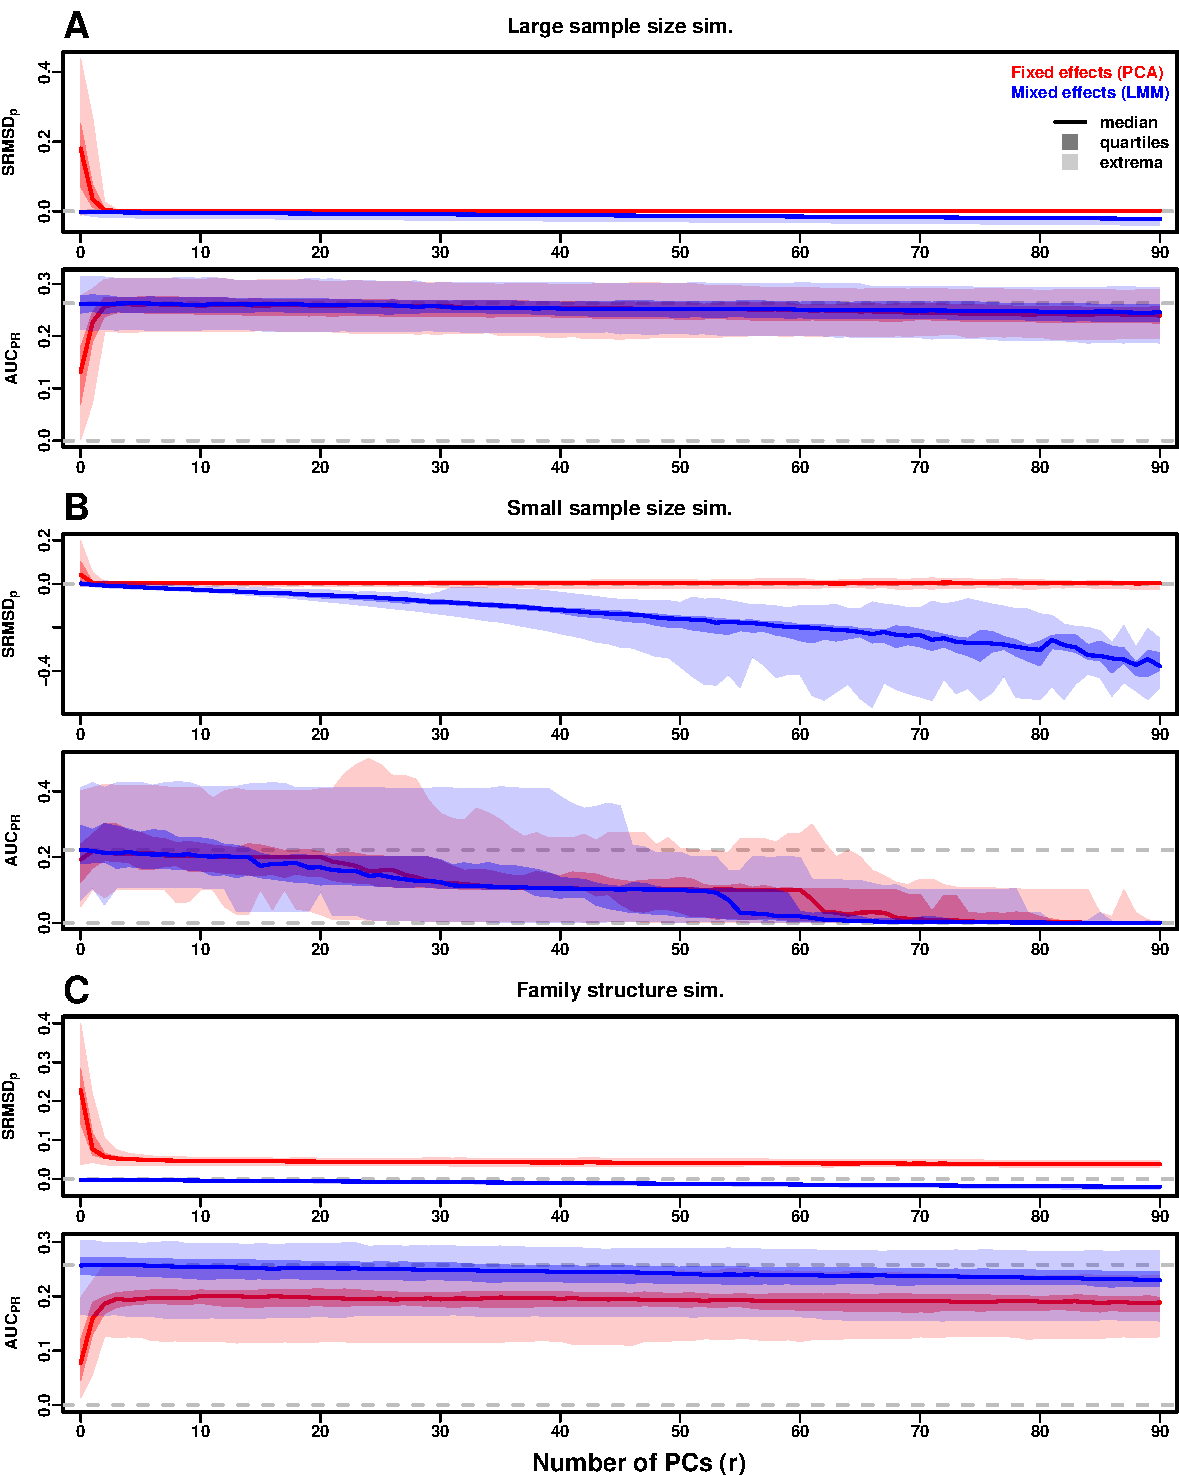
\includegraphics[width=\textwidth,height=\textheight,keepaspectratio]{rmsd-auc-sim.pdf}
  \caption{
    {\small 
      {\bf Evaluations in admixture simulations.}
      Traits simulated from \textit{random coefficients} model, otherwise the same as \cref{fig:rmsd-auc-sim}.
    }
  }
  \label{fig:rmsd-auc-sim-rc}
\end{figure}

\begin{figure}[bp!]
  \centering
  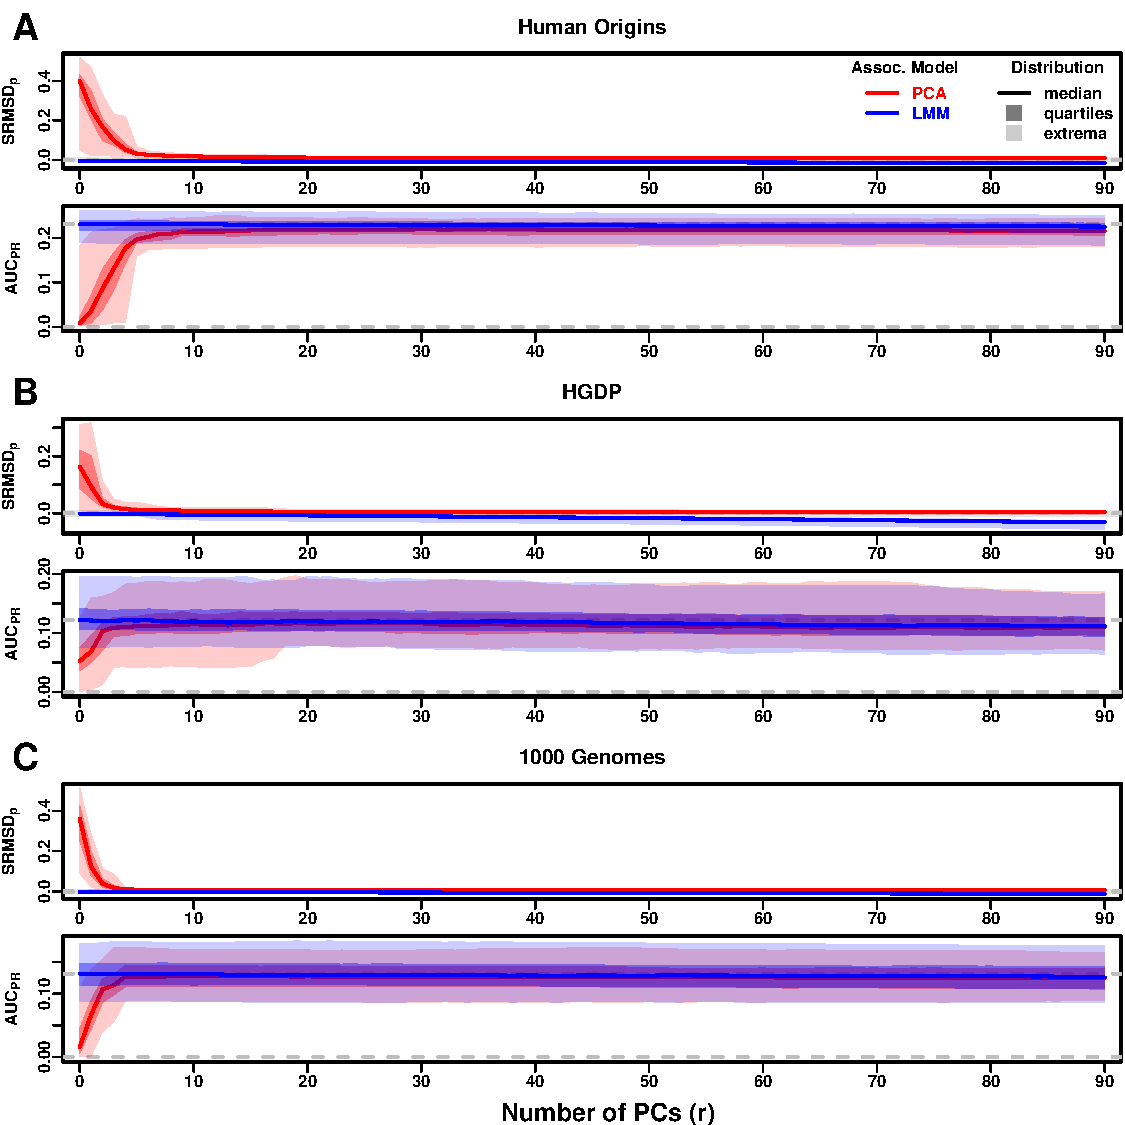
\includegraphics[width=\textwidth,height=\textheight,keepaspectratio]{rmsd-auc-real.pdf}
  \caption{
    {\small 
      {\bf Evaluations in real human genotype datasets.}
      Traits simulated from \textit{random coefficients} model, otherwise the same as \cref{fig:rmsd-auc-real}.
    }
  }
  \label{fig:rmsd-auc-real-rc}
\end{figure}

\begin{figure}[bp!]
  \centering
  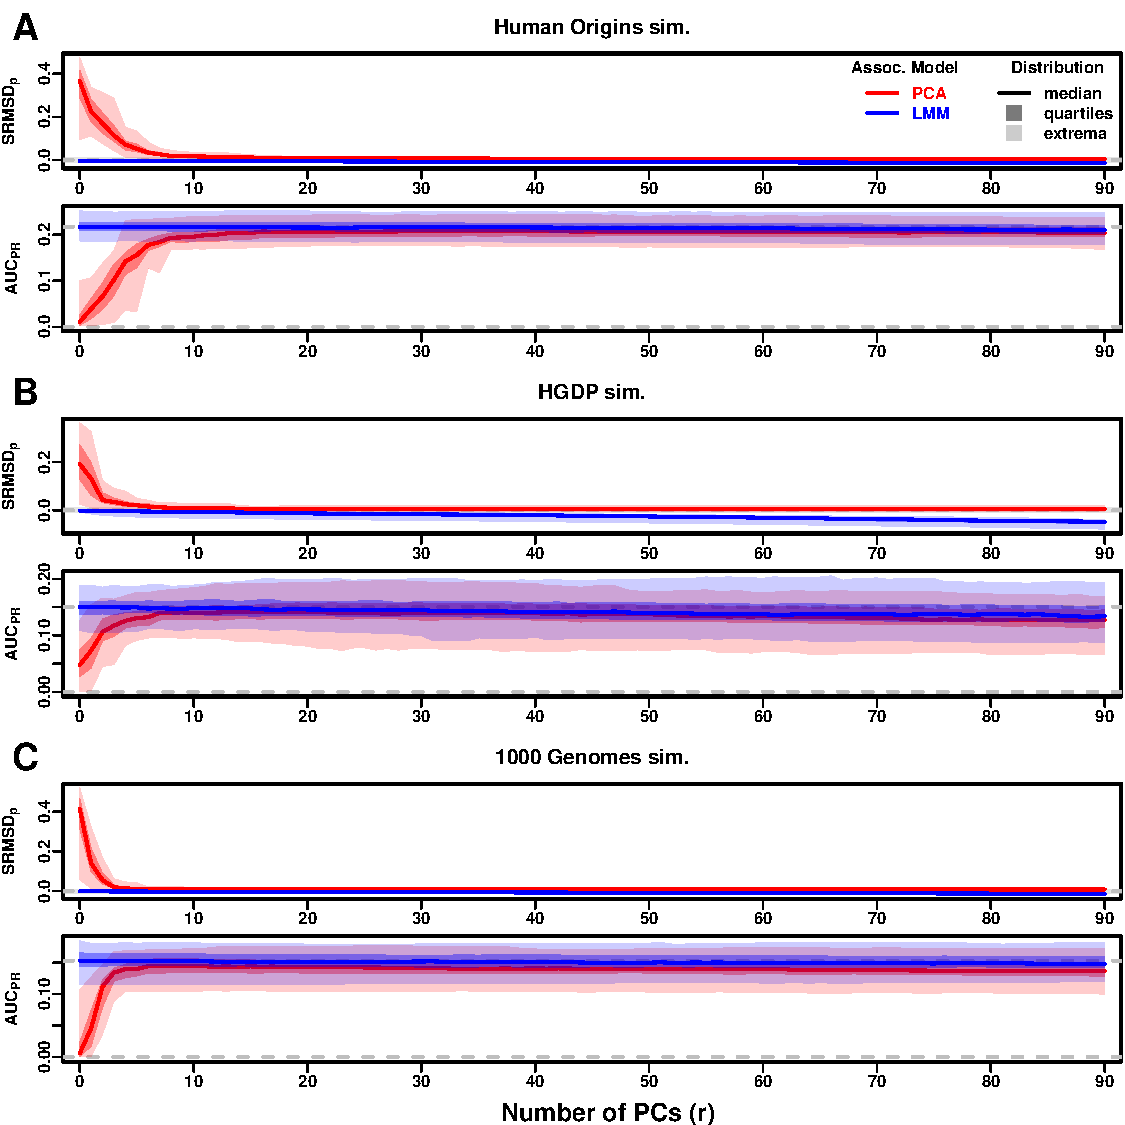
\includegraphics[width=\textwidth,height=\textheight,keepaspectratio]{rmsd-auc-real-sim.pdf}
  \caption{
    {\small 
      {\bf Evaluations in tree simulations fit to human data.}
      Traits simulated from \textit{random coefficients} model, otherwise the same as \cref{fig:rmsd-auc-real-sim}.
    }
  }
  \label{fig:rmsd-auc-real-sim-rc}
\end{figure}



\end{document}